% Options for packages loaded elsewhere
% Options for packages loaded elsewhere
\PassOptionsToPackage{unicode}{hyperref}
\PassOptionsToPackage{hyphens}{url}
%
\documentclass[
  8pt,
  ignorenonframetext,
  aspectratio=169,
  spanish,
]{beamer}
\newif\ifbibliography
\usepackage{pgfpages}
\setbeamertemplate{caption}[numbered]
\setbeamertemplate{caption label separator}{: }
\setbeamercolor{caption name}{fg=normal text.fg}
\beamertemplatenavigationsymbolsempty
% remove section numbering
\setbeamertemplate{part page}{
  \centering
  \begin{beamercolorbox}[sep=16pt,center]{part title}
    \usebeamerfont{part title}\insertpart\par
  \end{beamercolorbox}
}
\setbeamertemplate{section page}{
  \centering
  \begin{beamercolorbox}[sep=12pt,center]{section title}
    \usebeamerfont{section title}\insertsection\par
  \end{beamercolorbox}
}
\setbeamertemplate{subsection page}{
  \centering
  \begin{beamercolorbox}[sep=8pt,center]{subsection title}
    \usebeamerfont{subsection title}\insertsubsection\par
  \end{beamercolorbox}
}
% Prevent slide breaks in the middle of a paragraph
\widowpenalties 1 10000
\raggedbottom
\AtBeginPart{
  \frame{\partpage}
}
\AtBeginSection{
  \ifbibliography
  \else
    \frame{\sectionpage}
  \fi
}
\AtBeginSubsection{
  \frame{\subsectionpage}
}
\usepackage{iftex}
\ifPDFTeX
  \usepackage[T1]{fontenc}
  \usepackage[utf8]{inputenc}
  \usepackage{textcomp} % provide euro and other symbols
\else % if luatex or xetex
  \usepackage{unicode-math} % this also loads fontspec
  \defaultfontfeatures{Scale=MatchLowercase}
  \defaultfontfeatures[\rmfamily]{Ligatures=TeX,Scale=1}
\fi
\usepackage{lmodern}

\usetheme[]{metropolis}
\usecolortheme[]{default}
\usefonttheme[]{professionalfonts}
\ifPDFTeX\else
  % xetex/luatex font selection
\fi
% Use upquote if available, for straight quotes in verbatim environments
\IfFileExists{upquote.sty}{\usepackage{upquote}}{}
\IfFileExists{microtype.sty}{% use microtype if available
  \usepackage[]{microtype}
  \UseMicrotypeSet[protrusion]{basicmath} % disable protrusion for tt fonts
}{}
\makeatletter
\@ifundefined{KOMAClassName}{% if non-KOMA class
  \IfFileExists{parskip.sty}{%
    \usepackage{parskip}
  }{% else
    \setlength{\parindent}{0pt}
    \setlength{\parskip}{6pt plus 2pt minus 1pt}}
}{% if KOMA class
  \KOMAoptions{parskip=half}}
\makeatother

\usepackage{color}
\usepackage{fancyvrb}
\newcommand{\VerbBar}{|}
\newcommand{\VERB}{\Verb[commandchars=\\\{\}]}
\DefineVerbatimEnvironment{Highlighting}{Verbatim}{commandchars=\\\{\}}
% Add ',fontsize=\small' for more characters per line
\usepackage{framed}
\definecolor{shadecolor}{RGB}{241,243,245}
\newenvironment{Shaded}{\begin{snugshade}}{\end{snugshade}}
\newcommand{\AlertTok}[1]{\textcolor[rgb]{0.68,0.00,0.00}{#1}}
\newcommand{\AnnotationTok}[1]{\textcolor[rgb]{0.37,0.37,0.37}{#1}}
\newcommand{\AttributeTok}[1]{\textcolor[rgb]{0.40,0.45,0.13}{#1}}
\newcommand{\BaseNTok}[1]{\textcolor[rgb]{0.68,0.00,0.00}{#1}}
\newcommand{\BuiltInTok}[1]{\textcolor[rgb]{0.00,0.23,0.31}{#1}}
\newcommand{\CharTok}[1]{\textcolor[rgb]{0.13,0.47,0.30}{#1}}
\newcommand{\CommentTok}[1]{\textcolor[rgb]{0.37,0.37,0.37}{#1}}
\newcommand{\CommentVarTok}[1]{\textcolor[rgb]{0.37,0.37,0.37}{\textit{#1}}}
\newcommand{\ConstantTok}[1]{\textcolor[rgb]{0.56,0.35,0.01}{#1}}
\newcommand{\ControlFlowTok}[1]{\textcolor[rgb]{0.00,0.23,0.31}{\textbf{#1}}}
\newcommand{\DataTypeTok}[1]{\textcolor[rgb]{0.68,0.00,0.00}{#1}}
\newcommand{\DecValTok}[1]{\textcolor[rgb]{0.68,0.00,0.00}{#1}}
\newcommand{\DocumentationTok}[1]{\textcolor[rgb]{0.37,0.37,0.37}{\textit{#1}}}
\newcommand{\ErrorTok}[1]{\textcolor[rgb]{0.68,0.00,0.00}{#1}}
\newcommand{\ExtensionTok}[1]{\textcolor[rgb]{0.00,0.23,0.31}{#1}}
\newcommand{\FloatTok}[1]{\textcolor[rgb]{0.68,0.00,0.00}{#1}}
\newcommand{\FunctionTok}[1]{\textcolor[rgb]{0.28,0.35,0.67}{#1}}
\newcommand{\ImportTok}[1]{\textcolor[rgb]{0.00,0.46,0.62}{#1}}
\newcommand{\InformationTok}[1]{\textcolor[rgb]{0.37,0.37,0.37}{#1}}
\newcommand{\KeywordTok}[1]{\textcolor[rgb]{0.00,0.23,0.31}{\textbf{#1}}}
\newcommand{\NormalTok}[1]{\textcolor[rgb]{0.00,0.23,0.31}{#1}}
\newcommand{\OperatorTok}[1]{\textcolor[rgb]{0.37,0.37,0.37}{#1}}
\newcommand{\OtherTok}[1]{\textcolor[rgb]{0.00,0.23,0.31}{#1}}
\newcommand{\PreprocessorTok}[1]{\textcolor[rgb]{0.68,0.00,0.00}{#1}}
\newcommand{\RegionMarkerTok}[1]{\textcolor[rgb]{0.00,0.23,0.31}{#1}}
\newcommand{\SpecialCharTok}[1]{\textcolor[rgb]{0.37,0.37,0.37}{#1}}
\newcommand{\SpecialStringTok}[1]{\textcolor[rgb]{0.13,0.47,0.30}{#1}}
\newcommand{\StringTok}[1]{\textcolor[rgb]{0.13,0.47,0.30}{#1}}
\newcommand{\VariableTok}[1]{\textcolor[rgb]{0.07,0.07,0.07}{#1}}
\newcommand{\VerbatimStringTok}[1]{\textcolor[rgb]{0.13,0.47,0.30}{#1}}
\newcommand{\WarningTok}[1]{\textcolor[rgb]{0.37,0.37,0.37}{\textit{#1}}}

\usepackage{longtable,booktabs,array}
\usepackage{calc} % for calculating minipage widths
\usepackage{caption}
% Make caption package work with longtable
\makeatletter
\def\fnum@table{\tablename~\thetable}
\makeatother
\usepackage{graphicx}
\makeatletter
\newsavebox\pandoc@box
\newcommand*\pandocbounded[1]{% scales image to fit in text height/width
  \sbox\pandoc@box{#1}%
  \Gscale@div\@tempa{\textheight}{\dimexpr\ht\pandoc@box+\dp\pandoc@box\relax}%
  \Gscale@div\@tempb{\linewidth}{\wd\pandoc@box}%
  \ifdim\@tempb\p@<\@tempa\p@\let\@tempa\@tempb\fi% select the smaller of both
  \ifdim\@tempa\p@<\p@\scalebox{\@tempa}{\usebox\pandoc@box}%
  \else\usebox{\pandoc@box}%
  \fi%
}
% Set default figure placement to htbp
\def\fps@figure{htbp}
\makeatother



\ifLuaTeX
\usepackage[bidi=basic]{babel}
\else
\usepackage[bidi=default]{babel}
\fi
% get rid of language-specific shorthands (see #6817):
\let\LanguageShortHands\languageshorthands
\def\languageshorthands#1{}


\setlength{\emergencystretch}{3em} % prevent overfull lines

\providecommand{\tightlist}{%
  \setlength{\itemsep}{0pt}\setlength{\parskip}{0pt}}



 


\AtBeginDocument{\footnotesize}
\usepackage{etoolbox}
\usepackage{colortbl}
% Glifo prima (′, Parte 3) ausente en la fuente de metropolis.
% unicode-math hace math-activo el carácter en begin-document,
% así que su redefinición debe ir también en AtBeginDocument.
\usepackage{newunicodechar}
\AtBeginDocument{\newunicodechar{′}{\ensuremath{{}^{\prime}}}}
% Filete fino gris entre filas del cuerpo de las tablas;
% lo inyecta row-rules.lua en la salida beamer.
\newcommand{\lightrowrule}{\arrayrulecolor{black!25}\specialrule{0.4pt}{1pt}{1pt}\arrayrulecolor{black}}
\AtBeginEnvironment{Highlighting}{\scriptsize}
% Divisor de parte: contenido de una página plana que replica la
% portada metropolis (título grande + filete naranja), distinta de
% las páginas de sección. Lo emite roadmap.lua (#3 = línea de partes).
\newcommand{\partdividercontent}[3]{%
  \vfill
  {\color{mDarkTeal}\scriptsize\bfseries\MakeUppercase{#1}\par}
  \vspace{0.7em}
  {\usebeamerfont{title}\usebeamercolor[fg]{title}#2\par}
  \vspace{0.5em}
  {\color{mLightBrown}\rule{\textwidth}{0.05em}}
  \vspace{1.2em}
  #3
  \vfill}
% Mapa de progreso en las páginas de sección: roadmap.lua define
% \roadmapcontent antes de cada \section y la plantilla «section
% page» (adaptada de la variante progressbar de metropolis) lo
% imprime en lugar del título, sobre la barra de progreso.
\newcommand{\roadmapcontent}{}
\makeatletter
\setbeamertemplate{section page}{
  \centering
  % 0.8\textwidth (metropolis usa 22em): el mapa cabe en una línea.
  \begin{minipage}{0.8\textwidth}
    \raggedright
    \usebeamercolor[fg]{section title}
    \usebeamerfont{section title}
    % Sin \insertsectionhead: el mapa identifica la sección activa.
    \roadmapcontent
    \vspace{0.6em}
    \usebeamertemplate*{progress bar in section page}
    \par
  \end{minipage}
  \par
  \vspace{\baselineskip}
}
\makeatother
% Cierre «Agradecimientos»: fondo teal a página completa vía TikZ
% dentro de un frame [plain] normal. No se usa el [standout] de
% metropolis: con la plantilla beamer de Quarto su \begingroup
% queda sin cerrar (\end occurred inside a group) y el lienzo
% oscuro contamina los frames posteriores.
\usepackage{tikz}
\definecolor{SlateTealDeck}{HTML}{2D6A7A}
\makeatletter
\@ifpackageloaded{tcolorbox}{}{\usepackage[skins,breakable]{tcolorbox}}
\@ifpackageloaded{fontawesome5}{}{\usepackage{fontawesome5}}
\definecolor{quarto-callout-color}{HTML}{909090}
\definecolor{quarto-callout-note-color}{HTML}{0758E5}
\definecolor{quarto-callout-important-color}{HTML}{CC1914}
\definecolor{quarto-callout-warning-color}{HTML}{EB9113}
\definecolor{quarto-callout-tip-color}{HTML}{00A047}
\definecolor{quarto-callout-caution-color}{HTML}{FC5300}
\definecolor{quarto-callout-color-frame}{HTML}{acacac}
\definecolor{quarto-callout-note-color-frame}{HTML}{4582ec}
\definecolor{quarto-callout-important-color-frame}{HTML}{d9534f}
\definecolor{quarto-callout-warning-color-frame}{HTML}{f0ad4e}
\definecolor{quarto-callout-tip-color-frame}{HTML}{02b875}
\definecolor{quarto-callout-caution-color-frame}{HTML}{fd7e14}
\makeatother
\makeatletter
\@ifpackageloaded{caption}{}{\usepackage{caption}}
\AtBeginDocument{%
\ifdefined\contentsname
  \renewcommand*\contentsname{Tabla de contenidos}
\else
  \newcommand\contentsname{Tabla de contenidos}
\fi
\ifdefined\listfigurename
  \renewcommand*\listfigurename{Listado de Figuras}
\else
  \newcommand\listfigurename{Listado de Figuras}
\fi
\ifdefined\listtablename
  \renewcommand*\listtablename{Listado de Tablas}
\else
  \newcommand\listtablename{Listado de Tablas}
\fi
\ifdefined\figurename
  \renewcommand*\figurename{Figura}
\else
  \newcommand\figurename{Figura}
\fi
\ifdefined\tablename
  \renewcommand*\tablename{Tabla}
\else
  \newcommand\tablename{Tabla}
\fi
}
\@ifpackageloaded{float}{}{\usepackage{float}}
\floatstyle{ruled}
\@ifundefined{c@chapter}{\newfloat{codelisting}{h}{lop}}{\newfloat{codelisting}{h}{lop}[chapter]}
\floatname{codelisting}{Listado}
\newcommand*\listoflistings{\listof{codelisting}{Listado de Listados}}
\makeatother
\makeatletter
\makeatother
\makeatletter
\@ifpackageloaded{caption}{}{\usepackage{caption}}
\@ifpackageloaded{subcaption}{}{\usepackage{subcaption}}
\makeatother

\usepackage{bookmark}
\IfFileExists{xurl.sty}{\usepackage{xurl}}{} % add URL line breaks if available
\urlstyle{same}
\hypersetup{
  pdftitle={Concurso de acceso a Catedrático de Universidad},
  pdfauthor={Candidato: Juan de Dios Montoro Pons},
  pdflang={es},
  hidelinks,
  pdfcreator={LaTeX via pandoc}}


\title{Concurso de acceso a Catedrático de Universidad}
\subtitle{Área de conocimiento: Métodos Cuantitativos para la Economía y
la Empresa \newline \footnotesize Plaza 573 · Código 78/2026 ·
Resolución de 23 de junio de 2026 de la Universitat de València}
\author{Candidato: Juan de Dios Montoro Pons}
\date{24 septiembre 2026}

\begin{document}
\frame{\titlepage}


\begin{frame}
\partdividercontent{Parte 1 de 3}{Currículum}{{\scriptsize \mbox{\color{mDarkTeal}\bfseries Parte 1 · Currículum}\quad \mbox{\color{black!40}Parte 2 · Propuesta docente}\quad \mbox{\color{black!40}Parte 3 · Propuesta investigadora: Creative collaborations}\par}}

\note{Con la venia de la comisión, comienzo la presentación del
ejercicio para el concurso al cuerpo de catedráticos de universidad
convocado por la Universidad de Valencia, plaza 573.

Siguiendo las directrices de la convocatoria, presento en primer lugar
mi curriculum vitae.}
\end{frame}

\begin{frame}{Trayectoria académica: evolución}
\phantomsection\label{trayectoria-acaduxe9mica-evoluciuxf3n}
~


\includegraphics[width=0.96\linewidth,height=\textheight,keepaspectratio]{presentacion_ejercicio_files/mediabag/figures/fig_timeline.pdf}

\note{La línea temporal resume mi trayectoria en la Universitat de
València, desde la finalización de la licenciatura en Ciencias
Económicas y Empresariales en 1991 hasta la acreditación a catedrático
de universidad por la ANECA en octubre de 2024.

En la primera etapa (de formación y estabilización) defiendo la tesis
doctoral en 1996, obtengo la plaza de ayudante en 1997 en el área de
Economía Aplicada, la titularidad de escuela en 2002, y la habilitación
nacional a titular de universidad en el concurso celebrado en la
universidad de Alcalá de Henares en 2004 con la que accedo a la plaza en
2005.

La segunda etapa (de orientación internacional) comienza con la
adscripción al área de Métodos Cuantitativos en 2007 concentrando la
coordinación del título de ADE/GEDE, el proyecto ATLANTIS de la UE y la
fundación y vicepresidencia de IMBRA.

En la tercera, desde 2016, de consolidación y liderazgo, obtengo la
evaluación positiva del tercer y cuarto sexenio de investigación, dirijo
el grupo de investigación CREAMARKT y el grupo consolidado de innovación
docente MULTIATC.}

\gdef\roadmapcontent{{\scriptsize \mbox{\color{mDarkTeal}\bfseries Parte 1 · Currículum}\quad \mbox{\color{black!40}Parte 2 · Propuesta docente}\quad \mbox{\color{black!40}Parte 3 · Propuesta investigadora: Creative collaborations}\par}
\vspace{0.8em}
{\large \mbox{\color{mDarkTeal}\bfseries Investigación y transferencia}~· \mbox{\color{black!40}Docencia}~· \mbox{\color{black!40}Dirección y liderazgo}\par}}
\end{frame}

\section{Investigación y
transferencia}\label{investigaciuxf3n-y-transferencia}

\note{La exposición sigue el orden del currículum: investigación y
transferencia, docencia, y finalmente, gestión, dirección de equipos y
liderazgo.

Empiezo por la investigación.}

\begin{frame}[shrink]{Trayectoria investigadora}
\phantomsection\label{trayectoria-investigadora}
~

\begin{longtable}[]{@{}
  >{\raggedright\arraybackslash}p{(\linewidth - 4\tabcolsep) * \real{0.2273}}
  >{\raggedright\arraybackslash}p{(\linewidth - 4\tabcolsep) * \real{0.4545}}
  >{\raggedright\arraybackslash}p{(\linewidth - 4\tabcolsep) * \real{0.3182}}@{}}
\toprule\noalign{}
\begin{minipage}[b]{\linewidth}\raggedright
Etapa
\end{minipage} & \begin{minipage}[b]{\linewidth}\raggedright
Trabajos representativos
\end{minipage} & \begin{minipage}[b]{\linewidth}\raggedright
Principales coautores
\end{minipage} \\
\midrule\noalign{}
\endhead
\bottomrule\noalign{}
\endlastfoot
\textbf{Economía computacional} (1995--2003) & Tesis doctoral
``Simulación y Detección de Caos Macroeconómico'' (1996) · Capítulos en
\emph{Mathematics with Vision} (CMP, 1995) e \emph{Innovations in
Mathematics} (CMP, 1997) · \emph{Journal of Macroeconomics} (1998) &
José V. Paz-García \\ \lightrowrule
\textbf{Elección pública} (1998--2010) & Capítulos en \emph{Methods and
Moral in Constitutional Economics. Essays in Honour of James M.
Buchanan} (Springer, 2001) y en \emph{Constitutional Economics and
Public Institutions} (Edward Elgar, 2013) · \emph{CIRIEC-España} (2000)
· \emph{Constitutional Political Economy} (2001) · \emph{Computational
Economics} (2003) & Miguel Puchades-Navarro José Casas-Pardo \\ \lightrowrule
\textbf{Economía de la cultura y consumo cultural} (2008--) & Transición
vía propiedad intelectual \(\to\) participación cultural e industrias
creativas y \emph{big data} : \emph{European Journal of Law and
Economics} (2008) · \emph{Journal of Cultural Economics} (2011, 2018) ·
\emph{Poetics} (2020, 2025) · \emph{Empirical Economics} (2023) & Manuel
Cuadrado-García María Caballer-Tarazona María Luisa Palma-Martos \\ \lightrowrule
\end{longtable}

\note{La tabla ordena la trayectoria investigadora en tres etapas con
algún solapamiento, los trabajos representativos y los principales
coautores.

La primera, de 1995 a 2003, centrada en economía computacional, se
articula en torno a la elaboración de la tesis doctoral sobre simulación
y detección de caos macroeconómico, dirigida por el profesor José
Vicente Paz, que obtuvo la calificación de sobresaliente cum laude y que
da lugar a dos capítulos en la editorial Computational Mechanics
Publications y un artículo en el Journal of Macroeconomics (revista
JCR).

La segunda, de 1998 a 2010, incorpora la teoría de la elección pública
con diversos trabajos junto a los profesores Miguel Puchades-Navarro y
José Casas-Pardo: artículos publicados en CIRIEC-España, Constitutional
Political Economy, Computational Economics y capítulos en el homenaje al
nobel James Buchanan en Springer o en el libro \textbf{Constitutional
Economics and Public Institutions} en Edward Elgar.

La tercera etapa, desde 2008, se orienta a la economía de la cultura e
industrias creativas. La transición entre estas dos últimas viene de la
investigación sobre propiedad intelectual, con resultados como el
artículo de 2008 en el European Journal of Law and Economics. Los
trabajos de esta línea se realizan junto al profesor Manuel
Cuadrado-García, y más recientemente las profesoras María
Caballer-Tarazona y María Luisa Palma-Martos, y en ellos se exploran
diversos aspectos de la participación cultural, las industrias creativas
y el big data, cuyos resultados se publican en revistas como el Journal
of Cultural Economics, Poetics o Empirical Economics.}
\end{frame}

\begin{frame}{Producción científica en cifras}
\phantomsection\label{producciuxf3n-cientuxedfica-en-cifras}
~

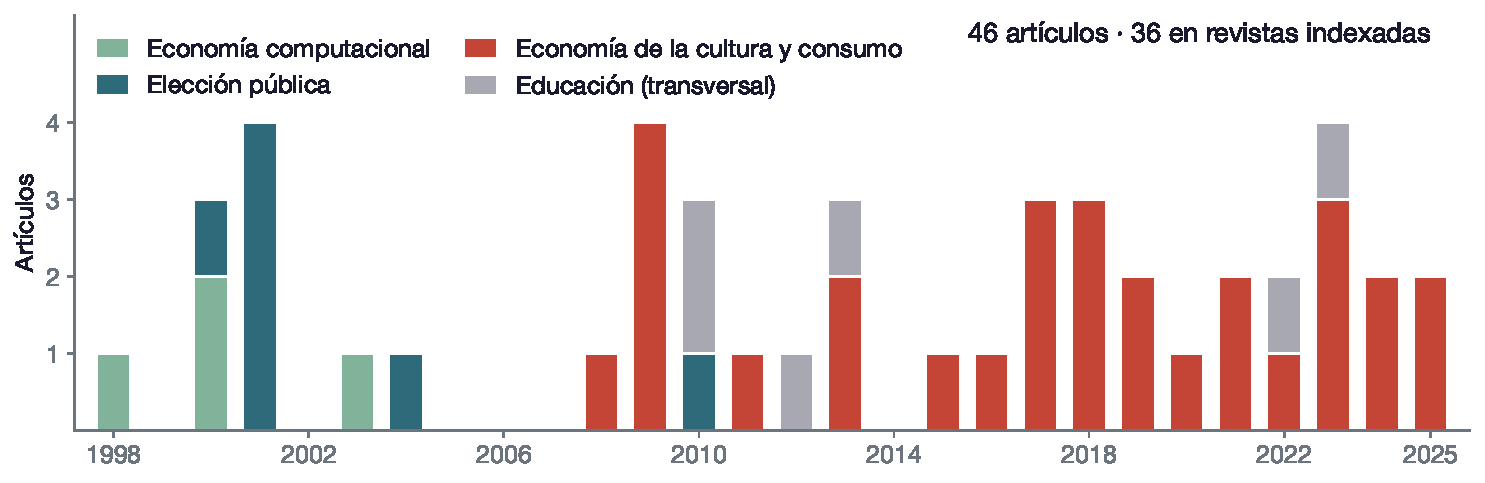
\includegraphics[width=0.88\linewidth,height=\textheight,keepaspectratio]{presentacion_ejercicio_files/mediabag/figures/fig_articulos_etapas.pdf}

\begin{longtable}[]{@{}
  >{\centering\arraybackslash}p{(\linewidth - 4\tabcolsep) * \real{0.3333}}
  >{\centering\arraybackslash}p{(\linewidth - 4\tabcolsep) * \real{0.3333}}
  >{\centering\arraybackslash}p{(\linewidth - 4\tabcolsep) * \real{0.3333}}@{}}
\toprule\noalign{}
\begin{minipage}[b]{\linewidth}\centering
Web of Science
\end{minipage} & \begin{minipage}[b]{\linewidth}\centering
Scopus
\end{minipage} & \begin{minipage}[b]{\linewidth}\centering
Google Scholar
\end{minipage} \\
\midrule\noalign{}
\endhead
\bottomrule\noalign{}
\endlastfoot
251 citas · h = 8 & 335 citas · h = 8 & 807 citas · h = 14 · i10 = 19 \\ \lightrowrule
\end{longtable}

\note{La diapositiva cuantifica la producción científica agrupada por
año y categoría junto con un resumen de los índices bibliométricos. Un
análisis de estos muestra una investigación con una serie ascendente de
citas (cerca del sesenta por ciento de las citas se ha recibido desde
2021) mayoritariamente externas (más del noventa por ciento) y que más
allá de la academia ha tenido impacto en documentos de política pública.

De ese conjunto selecciono ocho publicaciones por su relevancia.}
\end{frame}

\begin{frame}[shrink]{Publicaciones seleccionadas}
\phantomsection\label{publicaciones-seleccionadas}
~

\begin{longtable}[]{@{}
  >{\raggedright\arraybackslash}p{(\linewidth - 6\tabcolsep) * \real{0.3704}}
  >{\raggedright\arraybackslash}p{(\linewidth - 6\tabcolsep) * \real{0.2593}}
  >{\raggedright\arraybackslash}p{(\linewidth - 6\tabcolsep) * \real{0.1481}}
  >{\centering\arraybackslash}p{(\linewidth - 6\tabcolsep) * \real{0.2222}}@{}}
\toprule\noalign{}
\begin{minipage}[b]{\linewidth}\raggedright
Trabajo
\end{minipage} & \begin{minipage}[b]{\linewidth}\raggedright
Revista, año
\end{minipage} & \begin{minipage}[b]{\linewidth}\raggedright
Indicios
\end{minipage} & \begin{minipage}[b]{\linewidth}\centering
Citas (WoS · Scopus · GS)
\end{minipage} \\
\midrule\noalign{}
\endhead
\bottomrule\noalign{}
\endlastfoot
\textbf{Live and prerecorded popular music consumption} & \emph{J. of
Cultural Economics}, 2011 & JCR \textbf{Q2} (Economics) & 44 · 54 ·
124 \\ \lightrowrule
\textbf{Religiosity and cultural consumption} & \emph{Int. J. of
Consumer Studies}, 2018 & JCR \textbf{Q1} (Business) & 23 · 27 · 40 \\ \lightrowrule
\textbf{From pirates to subscribers: 20 years of music consumption
research} & \emph{Int. J. of Consumer Studies}, 2021 & JCR \textbf{Q1}
(Business) & 20 · 25 · 37 \\ \lightrowrule
\textbf{Analyzing online search patterns of music festival tourists} &
\emph{Tourism Economics}, 2021 & JCR \textbf{Q1} (Economics) & 7 · 8 ·
12 \\ \lightrowrule
\textbf{Music festivals as mediators and their influence on consumer
awareness} & \emph{Poetics}, 2020 & JCR \textbf{Q1} (Sociology) & 4 · 6
· 20 \\ \lightrowrule
\textbf{``Let's make lots of money'': performance in the recorded music
sector} & \emph{J. of Cultural Economics}, 2018 & JCR \textbf{Q2}
(Economics) & 6 · 7 · 15 \\ \lightrowrule
\textbf{Assessing complementarities between live performances and
YouTube video streaming} & \emph{Empirical Economics}, 2023 & JCR
\textbf{Q2} (Economics) & 2 · 3 · 8 \\ \lightrowrule
\textbf{Arts and cultural consumption and diversity research: a
bibliometric analysis} & \emph{Poetics}, 2025 & JCR \textbf{Q1}
(Sociology) & -- · 1 · 3 \\ \lightrowrule
\end{longtable}

\note{Destaco el artículo de 2011 en el Journal of Cultural Economics al
tratarse del más citado del área en mi perfil, que versa sobre la
complementariedad del consumo de música grabada y vivo.

Un segundo bloque lo constituyen los artículos publicados en Poetics,
primer cuartil de sociología y referencia en sociología de la cultura:
en 2020 (festivales de música como \emph{gatekeepers}) y 2025 (análisis
de la literatura sobre consumo cultural y diversidad).

Finalmente, la publicación en 2021 en el International Journal of
Consumer Studies (primer cuartil de business) que revisa y sistematiza
veinte años de estudios sobre consumo de música y define la agenda
futura de investigación.}
\end{frame}

\begin{frame}[shrink]{Capítulos de libro}
\phantomsection\label{capuxedtulos-de-libro}
~

\begin{longtable}[]{@{}
  >{\raggedright\arraybackslash}p{(\linewidth - 2\tabcolsep) * \real{0.5714}}
  >{\raggedright\arraybackslash}p{(\linewidth - 2\tabcolsep) * \real{0.4286}}@{}}
\toprule\noalign{}
\begin{minipage}[b]{\linewidth}\raggedright
Capítulo
\end{minipage} & \begin{minipage}[b]{\linewidth}\raggedright
Obra · editorial, año
\end{minipage} \\
\midrule\noalign{}
\endhead
\bottomrule\noalign{}
\endlastfoot
\textbf{Evolution and learning in collective decision-making} & Homenaje
a J. M. Buchanan (\emph{Methods and Moral in Constitutional Economics})
· \textbf{Springer}, 2001 \\ \lightrowrule
\textbf{Empirical insights into recorded music consumer behavior and
copyright infringement} & \emph{Music and Law} · \textbf{Emerald},
2013 \\ \lightrowrule
\textbf{Regulator preferences and lobbying efforts in rent-seeking
contest} & \emph{Constitutional Economics and Public Institutions} ·
\textbf{Edward Elgar}, 2013 \\ \lightrowrule
\textbf{Copyright infringement and cultural participation} &
\emph{Digital Piracy: A Global, Multidisciplinary Account} ·
\textbf{Routledge}, 2018 \\ \lightrowrule
\textbf{Breaking the gender gap in Rap/Hip-Hop consumption} &
\emph{Music as Intangible Cultural Heritage} · \textbf{Springer},
2021 \\ \lightrowrule
\textbf{Digital participation and audience enlargement in classical and
popular music} & \emph{Digital Transformation in the Cultural and
Creative Industries} · \textbf{Routledge}, 2021 \\ \lightrowrule
\textbf{Measuring customer multi-sensory experience in live music} &
\emph{The Oxford Handbook of Arts and Cultural Management} ·
\textbf{Oxford University Press}, 2022 \\ \lightrowrule
\end{longtable}

Selección por editorial académica internacional · \textbf{29 capítulos y
libros} en total · 4 casos docentes en el manual \emph{Marketing Culture
and the Arts} (HEC Montréal) y sus ediciones francesas.

\note{Junto a los artículos, la segunda vía de publicación de resultados
han sido los capítulos de libro.

La proyección recoge siete capítulos seleccionados por la relevancia de
la editorial (todas en las primeras posiciones del índice SPI) entre
2001 y 2022, de los veintinueve capítulos y libros que constan en el
currículum.

Previa a su materialización como publicación, esta producción académica
se ha presentado y discutido de forma continuada en congresos y
conferencias.}
\end{frame}

\begin{frame}{Comunicaciones en congresos}
\phantomsection\label{comunicaciones-en-congresos}
~

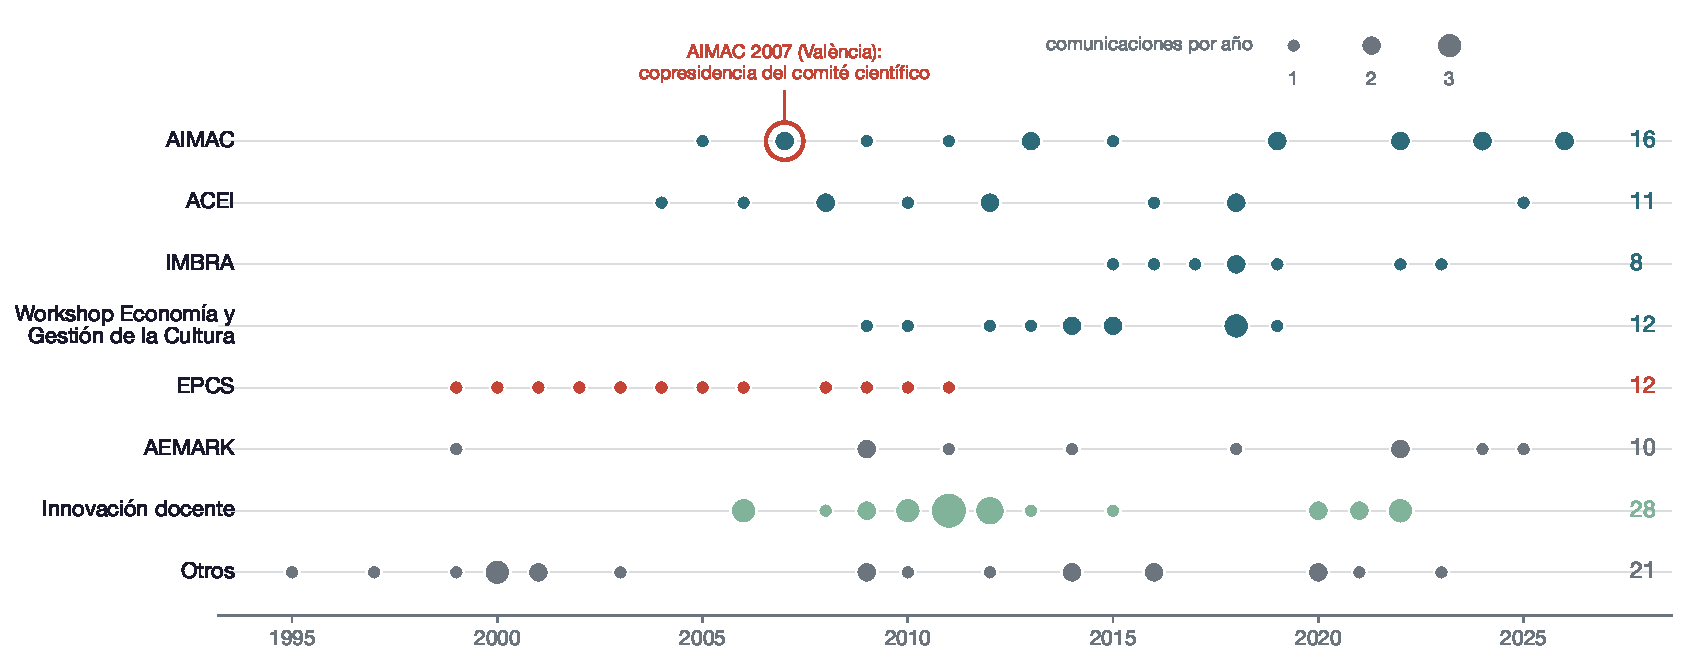
\includegraphics[width=1\linewidth,height=\textheight,keepaspectratio]{presentacion_ejercicio_files/mediabag/figures/fig_congresos_series.pdf}

Total: 118 ponencias · 92 de carácter internacional

\note{La figura ordena las comunicaciones a congresos, la mayor parte
internacionales, por organización y año.

En ella se observa una recurrencia y vigencia de la participación en las
conferencias de las principales asociaciones científicas del ámbito de
economía de la cultura y gestión cultural (como AIMAC, ACEI o IMBRA).}
\end{frame}

\begin{frame}{Proyectos de I+D+i en convocatoria pública}
\phantomsection\label{proyectos-de-idi-en-convocatoria-puxfablica}
~

\begin{longtable}[]{@{}
  >{\raggedright\arraybackslash}p{(\linewidth - 6\tabcolsep) * \real{0.4167}}
  >{\raggedright\arraybackslash}p{(\linewidth - 6\tabcolsep) * \real{0.2500}}
  >{\centering\arraybackslash}p{(\linewidth - 6\tabcolsep) * \real{0.1667}}
  >{\centering\arraybackslash}p{(\linewidth - 6\tabcolsep) * \real{0.1667}}@{}}
\toprule\noalign{}
\begin{minipage}[b]{\linewidth}\raggedright
Proyecto
\end{minipage} & \begin{minipage}[b]{\linewidth}\raggedright
Convocatoria
\end{minipage} & \begin{minipage}[b]{\linewidth}\centering
Años
\end{minipage} & \begin{minipage}[b]{\linewidth}\centering
Participación
\end{minipage} \\
\midrule\noalign{}
\endhead
\bottomrule\noalign{}
\endlastfoot
Teoría del caos: evolución, predicción y control de sistemas &
Generalitat Valenciana (AE98-08) & 1998 & equipo \\ \lightrowrule
Deficiencias en el funcionamiento de las instituciones democráticas &
CICYT (SEC99-0592) & 1999--2003 & equipo \\ \lightrowrule
Teoría del caos: autoorganización y control de sistemas complejos & MCyT
(PGC2000-2390-E) & 2001--2002 & equipo \\ \lightrowrule
Protección del cliente y eficiencia en el sistema financiero (Ley
44/2002) & MCyT (SEC2003-05232) & 2003--2006 & equipo \\ \lightrowrule
Proyecto de colaboración interdisciplinar, bilingüe y virtual entre
universidades de la Unión Europea para la dinamización del proceso de
aprendizaje & Ministerio de Ciencia e Innovación & 2008--2009 &
equipo \\ \lightrowrule
MBA-TABSA · Transatlantic Business School Alliance & Comisión Europea
(EACEA) & 2010--2014 & IP \\ \lightrowrule
La regulación de la economía colaborativa & Plan Estatal
(DER2015-67613-R) & 2016--2019 & equipo \\ \lightrowrule
\end{longtable}

~

\note{Toda la actividad investigadora se ha apoyado en dos pilares para
su financiación: el primero los proyectos financiados.

Se muestran los proyectos en convocatoria pública, con la entidad
financiadora, los años y mi participación. Cabe subrayar la continuidad
que muestran y los tres niveles de convocatoria: autonómica, nacional y
europea. Me detengo en el proyecto ATLANTIS MBA-TABSA financiado por la
Comisión Europea entre 2010 y 2014 donde, en colaboración con
universidades europeas y norteamericanas, se analiza el impacto
académico de la movilidad del alumnado entre instituciones y se diseñan
mecanismos para incentivar los vinculos de investigación entre
académicos.}
\end{frame}

\begin{frame}[shrink]{Contratos y convenios de transferencia (art. 83
LOU / 60 LOSU)}
\phantomsection\label{contratos-y-convenios-de-transferencia-art.-83-lou-60-losu}
~

\begin{longtable}[]{@{}
  >{\raggedright\arraybackslash}p{(\linewidth - 6\tabcolsep) * \real{0.2857}}
  >{\raggedright\arraybackslash}p{(\linewidth - 6\tabcolsep) * \real{0.5000}}
  >{\centering\arraybackslash}p{(\linewidth - 6\tabcolsep) * \real{0.1071}}
  >{\raggedright\arraybackslash}p{(\linewidth - 6\tabcolsep) * \real{0.1071}}@{}}
\toprule\noalign{}
\begin{minipage}[b]{\linewidth}\raggedright
Entidad
\end{minipage} & \begin{minipage}[b]{\linewidth}\raggedright
Objeto
\end{minipage} & \begin{minipage}[b]{\linewidth}\centering
Años
\end{minipage} & \begin{minipage}[b]{\linewidth}\raggedright
Participación
\end{minipage} \\
\midrule\noalign{}
\endhead
\bottomrule\noalign{}
\endlastfoot
AVETID & Estudio de públicos del Festival Tercera Setmana & 2017--18 &
equipo \\ \lightrowrule
Francachela Teatro & Plan de patrocinio y premios del festival &
2018--19 & IP \\ \lightrowrule
AVETID & Estudio de públicos Tercera Setmana, 2ª edición & 2018--19 &
equipo \\ \lightrowrule
EXTREMUS Danza & Evaluación de proyecto artístico de inclusión social &
2019--20 & equipo \\ \lightrowrule
Francachela Teatro & Plan de patrocinio y premios del festival &
2020--21 & IP \\ \lightrowrule
Olympia Metropolitana & Estudio de públicos en contexto teatral &
2021--22 & IP \\ \lightrowrule
A más Soluciones Culturales & Distribución en artes escénicas & 2021--22
& IP \\ \lightrowrule
Generalitat Valenciana & Perfil y experiencia del visitante del CCCC &
2022--23 & IP \\ \lightrowrule
ICOM International & SENTOMUS, museums visitors research & 2023--24 &
IP \\ \lightrowrule
BIOPARC València & Estudio de visitantes & 2023--24 & equipo \\ \lightrowrule
\end{longtable}

~

Total: 16 contratos/convenios con el tejido cultural desde 2012 · IP en
6 · Actividad reconocida con el \textbf{sexenio de transferencia}
(2012--2017)

\note{El segundo pilar para la financiación de la actividad
investigadora ha venido de la transferencia con el sector cultural.

La dispositiva muestra los diez contratos y convenios más recientes con
el tejido cultural. En total son dieciséis desde 2012, seis de ellos
como investigador principal, una actividad que está reconocida con el
sexenio de transferencia del periodo 2012--2017.

Es importante señalar que la transferencia forma parte de la
investigación: estos convenios generan datos y preguntas que acaban en
publicaciones, como es el caso del artículo de 2022 en el Journal of
Homosexuality, segundo cuartil JCR, cuyo origen es el convenio con
Francachela Teatro.}
\end{frame}

\begin{frame}{Estancias de investigación}
\phantomsection\label{estancias-de-investigaciuxf3n}
~

\begin{longtable}[]{@{}
  >{\raggedright\arraybackslash}p{(\linewidth - 4\tabcolsep) * \real{0.5556}}
  >{\raggedright\arraybackslash}p{(\linewidth - 4\tabcolsep) * \real{0.3333}}
  >{\centering\arraybackslash}p{(\linewidth - 4\tabcolsep) * \real{0.1111}}@{}}
\toprule\noalign{}
\begin{minipage}[b]{\linewidth}\raggedright
Estancia
\end{minipage} & \begin{minipage}[b]{\linewidth}\raggedright
Financiación
\end{minipage} & \begin{minipage}[b]{\linewidth}\centering
Periodo
\end{minipage} \\
\midrule\noalign{}
\endhead
\bottomrule\noalign{}
\endlastfoot
Center for Study of Public Choice / J. Buchanan Center, George Mason
Univ. (EE. UU.) & Generalitat Valenciana & 1998 · 6 m \\ \lightrowrule
HEC, Université de Montréal (Canadá) & Universitat de València & 1999 ·
1 m \\ \lightrowrule
CREED, Universiteit van Amsterdam (Países Bajos) & Generalitat
Valenciana & 2001 · 4 m \\ \lightrowrule
HEC, Université de Montréal (Canadá) & Generalitat Valenciana & 2007 · 2
m \\ \lightrowrule
London School of Economics (Reino Unido) & Universitat de València &
2007 · 2 m \\ \lightrowrule
Institut für Kulturmanagement, Univ. für Musik und Darstellende Kunst
Wien (Austria) & Universitat de València & 2013 · 3 m \\ \lightrowrule
\end{longtable}

~

6 estancias oficiales · 5 países · ≈18 meses acumulados · Todas con
financiación competitiva (Generalitat Valenciana / Universitat de
València)

\note{Un aspecto adicional de la dimensión investigadora son las
estancias de investigación. En total he realizado seis estancias en
cinco centros distintos, todas con financiación competitiva, acumulando
un total de dieciocho meses.}
\end{frame}

\begin{frame}{Dirección de tesis doctorales}
\phantomsection\label{direcciuxf3n-de-tesis-doctorales}
~

\begin{longtable}[]{@{}
  >{\raggedright\arraybackslash}p{(\linewidth - 8\tabcolsep) * \real{0.2830}}
  >{\raggedright\arraybackslash}p{(\linewidth - 8\tabcolsep) * \real{0.1698}}
  >{\raggedright\arraybackslash}p{(\linewidth - 8\tabcolsep) * \real{0.2264}}
  >{\raggedright\arraybackslash}p{(\linewidth - 8\tabcolsep) * \real{0.0566}}
  >{\centering\arraybackslash}p{(\linewidth - 8\tabcolsep) * \real{0.2642}}@{}}
\toprule\noalign{}
\begin{minipage}[b]{\linewidth}\raggedright
Título
\end{minipage} & \begin{minipage}[b]{\linewidth}\raggedright
Autor
\end{minipage} & \begin{minipage}[b]{\linewidth}\raggedright
Afiliación
\end{minipage} & \begin{minipage}[b]{\linewidth}\raggedright
Año
\end{minipage} & \begin{minipage}[b]{\linewidth}\centering
Observaciones
\end{minipage} \\
\midrule\noalign{}
\endhead
\bottomrule\noalign{}
\endlastfoot
\emph{Segmentación y exhibición cinematográfica: un análisis del mercado
español basado en clases latentes} & Desamparados Lluch Tormos & CEU San
Pablo (Madrid) & 2017 & Sobresaliente \emph{cum laude} · Tesis doctoral
con mención internacional · \textbf{Premio Fundación SGAE de
Investigación 2018} \\ \lightrowrule
\emph{Analyzing the effect of the expanded servicescape on visitors'
satisfaction and loyalty in museums} & Piergiacomo Mion Dalle Carbonare
& Università Bocconi (Milán) & 2022 & Sobresaliente \emph{cum laude} ·
Tesis doctoral con mención internacional \\ \lightrowrule
\emph{Estudio de los determinantes, percepción y valoración del
consumidor de música clásica: una aproximación multidisciplinar} &
Ariadna Martin & Conservatorio Profesional de Música (Las Palmas de Gran
Canaria) & en curso & JCR en revisión \\ \lightrowrule
\emph{Consumer engagement and market structuring in the contemporary art
ecosystem: visitor behavior and responses to citywide interventions} &
Giuliano Picchi & MIT (Cambridge, MA) & en curso & Ponencia AIMAC2026 \\ \lightrowrule
\end{longtable}

\note{Cierro este bloque con la dirección de tesis doctorales, con dos
tesis leídas y dos en curso. Todas ellas dentro del programa de
doctorado en Marketing, con mención de calidad.

Las dos tesis leídas obtuvieron sobresaliente cum laude y mención
internacional. La de Desamparados Lluch, de 2017, sobre segmentación y
exhibición cinematográfica recibió además el Premio Fundación SGAE de
Investigación de 2018.

Las tesis en curso siguen la misma línea de investigación sobre mercados
e industrias culturales.

Con esto cierro investigación y transferencia y paso al bloque de
docencia.}

\gdef\roadmapcontent{{\scriptsize \mbox{\color{mDarkTeal}\bfseries Parte 1 · Currículum}\quad \mbox{\color{black!40}Parte 2 · Propuesta docente}\quad \mbox{\color{black!40}Parte 3 · Propuesta investigadora: Creative collaborations}\par}
\vspace{0.8em}
{\large \mbox{\color{black!40}Investigación y transferencia}~· \mbox{\color{mDarkTeal}\bfseries Docencia}~· \mbox{\color{black!40}Dirección y liderazgo}\par}}
\end{frame}

\section{Docencia}\label{docencia}

\note{}

\begin{frame}{Trayectoria docente}
\phantomsection\label{trayectoria-docente}
~

\begin{longtable}[]{@{}
  >{\raggedright\arraybackslash}p{(\linewidth - 4\tabcolsep) * \real{0.3333}}
  >{\raggedright\arraybackslash}p{(\linewidth - 4\tabcolsep) * \real{0.3333}}
  >{\raggedright\arraybackslash}p{(\linewidth - 4\tabcolsep) * \real{0.3333}}@{}}
\toprule\noalign{}
\begin{minipage}[b]{\linewidth}\raggedright
\textbf{Etapa}
\end{minipage} & \begin{minipage}[b]{\linewidth}\raggedright
\textbf{Asignaturas}
\end{minipage} & \begin{minipage}[b]{\linewidth}\raggedright
\textbf{Observaciones}
\end{minipage} \\
\midrule\noalign{}
\endhead
\bottomrule\noalign{}
\endlastfoot
\textbf{Economía Política (1997)} & Economía Política y Hacienda Pública
· Economía (Lic. en CC. y Técnicas Estadísticas) · Estadística e
Informática (CC. Empresariales) & Docencia impartida en castellano y
valenciano \\ \lightrowrule
\textbf{Métodos Cuantitativos · Modelización e Inferencia Estadística
(2006/07)} & Estadística I y II, Estadística Básica, Introducción a la
Inferencia Estadística & Integración de troncales en el grupo
internacional (ARA) con docencia impartida en inglés \\ \lightrowrule
\textbf{Métodos Cuantitativos · Aprendizaje Estadístico (2019)} & Grado
BIA: Datos No Estructurados, Técnicas Avanzadas de Predicción · Máster
CD: Inferencia Causal y Aprendizaje Máquina, Ciencia de Datos en Negocio
· Máster iMBA: Inteligencia de Negocios · Máster Economía: Big Data en
Economía & Aumento de la participación como docente en programas de
máster \\ \lightrowrule
\end{longtable}

~

Docencia en: 7 centros · 13 titulaciones · 18 asignaturas distintas (32
con formación no reglada) · docencia en castellano, inglés (C2) y
valenciano (C1) · 50\% de la docencia total es en inglés

\note{La tabla resume treinta años por etapas, con las asignaturas
impartidas. En términos agregados la docencia se distribuye en siete
centros, trece titulaciones y dieciocho asignaturas en castellano,
valenciano (acredito un nivel C1) e inglés (C2).

La primera etapa, desde 1997, en Economía Política (Facultad de Derecho)
se cierra con el cambio de área (a Métodos Cuantitativos) en el curso
2006-2007. En esta segunda etapa imparto las materias de estadística
introductoria e inferencia en inglés.

En la tercera, desde 2019 incorporo el aprendizaje estadístico a la
docencia. Imparto en esta etapa Datos No Estructurados y Técnicas
Avanzadas de Predicción en el grado en Inteligencia y Analítica de
Negocios y cuatro asignaturas de máster, entre ellas Inferencia Causal y
Aprendizaje Máquina en el máster en Ciencia de Datos y Big Data en
Economía en el máster en Economía.}
\end{frame}

\begin{frame}{Docencia reglada}
\phantomsection\label{docencia-reglada}
~

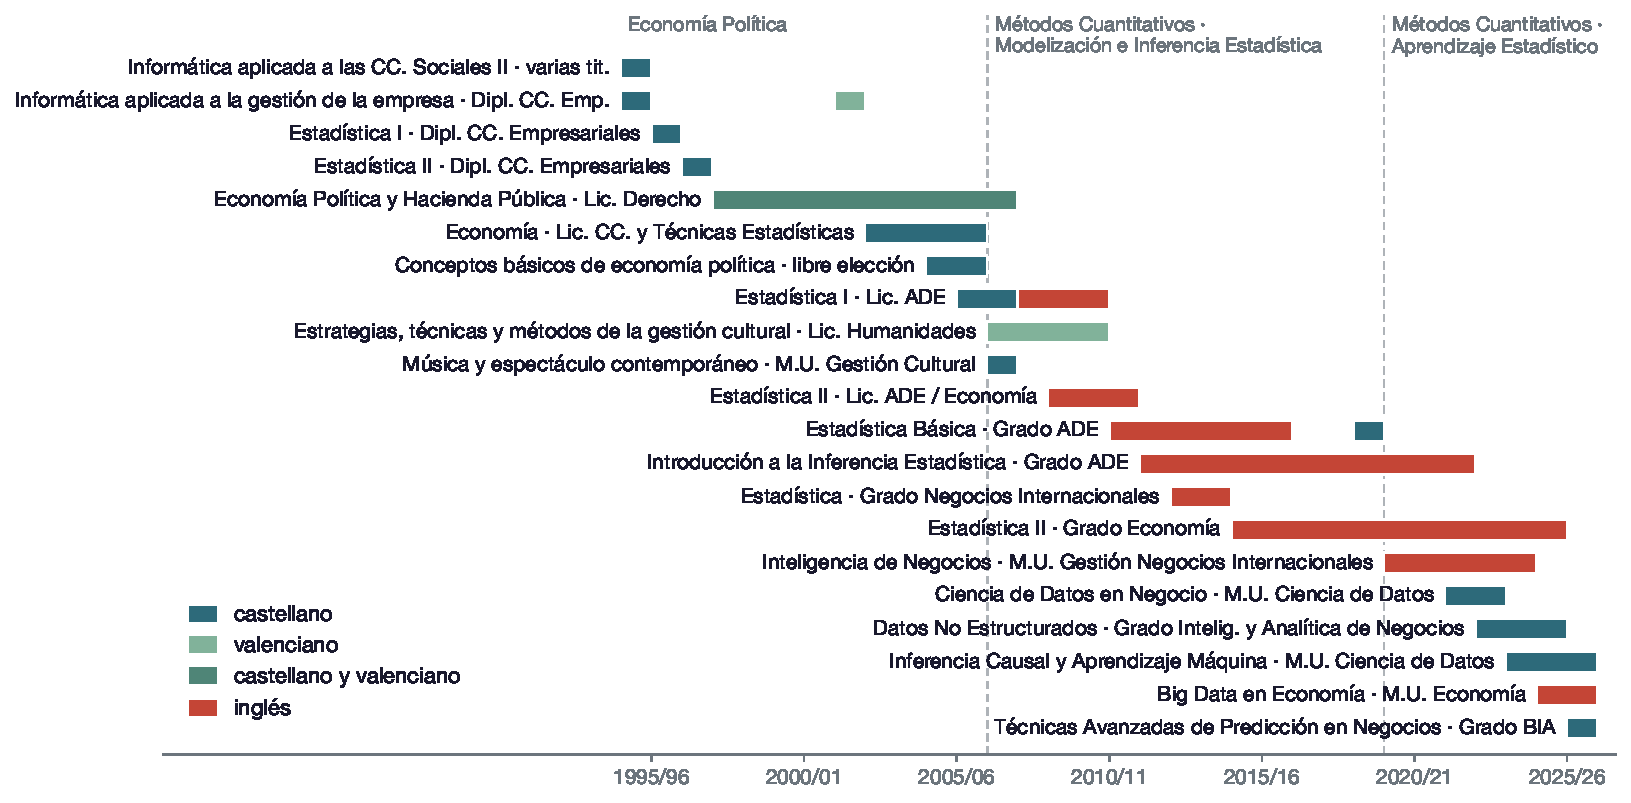
\includegraphics[width=1\linewidth,height=\textheight,keepaspectratio]{presentacion_ejercicio_files/mediabag/figures/fig_docencia_diversidad.pdf}

\note{La figura muestra todas las asignaturas impartidas por etapas e
idiomas.

Subrayar el peso de las clases en inglés que supone el 50\% del total
con mi incorporación en el año 2007 al grupo internacional, una apuesta
desarrollada por el equipo decanal de la Facultat liderado por Trinidad
Casasús Estellés.}
\end{frame}

\begin{frame}{Docencia internacional}
\phantomsection\label{docencia-internacional}
~

\begin{longtable}[]{@{}
  >{\raggedright\arraybackslash}p{(\linewidth - 4\tabcolsep) * \real{0.3200}}
  >{\raggedright\arraybackslash}p{(\linewidth - 4\tabcolsep) * \real{0.5200}}
  >{\raggedright\arraybackslash}p{(\linewidth - 4\tabcolsep) * \real{0.1600}}@{}}
\toprule\noalign{}
\begin{minipage}[b]{\linewidth}\raggedright
Destino / centro
\end{minipage} & \begin{minipage}[b]{\linewidth}\raggedright
Asignatura
\end{minipage} & \begin{minipage}[b]{\linewidth}\raggedright
Año(s)
\end{minipage} \\
\midrule\noalign{}
\endhead
\bottomrule\noalign{}
\endlastfoot
State University of New York at Albany & The World Trade System and the
Millenium Round · The Art of Managing Finance II (grado) & 2000 \\ \lightrowrule
London School of Economics and Political Science & Seminario ``Economía
y Música --- Análisis y Perspectivas de la Industria'' & 2007 \\ \lightrowrule
University of Hertfordshire & Managing the Small Business in the Music
Industry (grado) & 2011 \\ \lightrowrule
University of North Florida & Econometrics (grado) & 2013 \\ \lightrowrule
University of North Carolina at Wilmington & Statistics · International
Marketing (grado) & 2013 \\ \lightrowrule
Universidad de Buenos Aires & Seminario ``Información y toma de
decisiones en gestión cultural'' (maestría) & 2013 \\ \lightrowrule
Hochschule Bremen & Statistik I --- Quantitative Methoden (grado) &
2018 \\ \lightrowrule
International Graduate Center (Bremen) & Global Economics (MBA) & 2018 ·
2019 \\ \lightrowrule
\end{longtable}

~

\textbf{Estancias docentes}: 8 estancias oficiales · Docencia en
\textbf{programas} grado y posgrado

\note{Mi perfil docente se completa con la experiencia desarrollada en
otras instituciones universitarias. Se recogen aquí siete estancias
oficiales, con docencia en titulaciones de grado y posgrado, realizadas
entre 2000 y 2019.}
\end{frame}

\begin{frame}{Evaluación de la docencia}
\phantomsection\label{evaluaciuxf3n-de-la-docencia}
~


\includegraphics[width=0.92\linewidth,height=\textheight,keepaspectratio]{presentacion_ejercicio_files/mediabag/figures/fig_docentia.pdf}

\textbf{5 quinquenios} (29 cursos con evaluación positiva) · serie de
valoraciones ascendente, estable por encima de \textbf{4,3} desde 2017
(máximo 4,78 en 2023-24).

\note{La evaluación docente, útil para revisar y mejorar nuestra
actividad, se recoge aquí a través del programa DOCENTIA para
2017--2021, con la calificación de excelente en el nivel avanzado y la
máxima puntuación (200 puntos), y los informes anuales de evaluación de
1996 a 2024.

La serie temporal de la valoración media del alumnado muestra una
tendencia ascendente, se mantiene por encima de cuatro desde 2017 y
alcanza un máximo de 4,78 en el curso 2023--2024.}
\end{frame}

\begin{frame}[shrink]{Innovación docente}
\phantomsection\label{innovaciuxf3n-docente}
~

\begin{longtable}[]{@{}
  >{\raggedright\arraybackslash}p{(\linewidth - 2\tabcolsep) * \real{0.2000}}
  >{\raggedright\arraybackslash}p{(\linewidth - 2\tabcolsep) * \real{0.8000}}@{}}
\toprule\noalign{}
\begin{minipage}[b]{\linewidth}\raggedright
Tipo de Actividad
\end{minipage} & \begin{minipage}[b]{\linewidth}\raggedright
Descripción
\end{minipage} \\
\midrule\noalign{}
\endhead
\bottomrule\noalign{}
\endlastfoot
\textbf{Grupo de innovación} & Grupo ``Multi-aprendizaje,
transversalidad y creatividad (MULTI-ATC)'' --- co-director · Mención de
grupo consolidado en 2023 (renovada en 2026) · Continuidad del grupo
``Innova multidisciplinar'' (2009--2012). \\ \lightrowrule
\textbf{Proyectos dirigidos} & Proyectos dirigidos como IP: ``Jornada
docente transversal y solidaria'' (2021/22) · ``Investigación b-smart y
aprendizaje basado en un proyecto en un centro cultural'' (2022/23) ·
``Danza, salud e investigación'' (2024/25). \\ \lightrowrule
\textbf{Comunicaciones} & Comunicaciones (28): series recurrentes CIDUI
(2006--2012) · Trobades/Jornades d'Innovació Educativa UV (2010--2022) ·
Xarxes--REDES-INNOVAESTIC (2009--2021) · WCES (2010, 2012) · Congreso
Internacional de Innovación Docente (2022). \\ \lightrowrule
\textbf{Publicaciones} & Publicaciones: Procedia --- Social and
Behavioral Sciences (2010 --- derivada del piloto en línea con la LSE y
la más citada del perfil, 223 citas GS --- y 2012) · Rev.~Iberoamericana
de Educación (2010) · World J. on Educational Technology (2013) · RIEJS
(2022) · capítulo en Experiencias de Innovación Docente en Estadística
(2011). \\ \lightrowrule
\end{longtable}

~

14 \textbf{proyectos} (3 como IP) · Co-director del \textbf{grupo de
innovación consolidado} (mención 2023, renovada 2026) · 28
\textbf{comunicaciones} en congresos y jornadas ·
\textbf{Publicaciones}: 5 artículos + 1 capítulo

\note{Esa evolución ha ido pareja a la actividad y los proyectos en
innovación educativa, que se resumen en:

\begin{enumerate}
\tightlist
\item
  catorce proyectos (tres como investigador principal)\\
\item
  la codirección de un grupo de innovación consolidado (reconocido en
  2023 y renovado en 2026),\\
\item
  veintiocho comunicaciones en encuentros de referencia, como CIDUI y
  Redes-INNOVAESTIC.
\item
  y cinco artículos más un capítulo de libro.\\
\end{enumerate}}

\gdef\roadmapcontent{{\scriptsize \mbox{\color{mDarkTeal}\bfseries Parte 1 · Currículum}\quad \mbox{\color{black!40}Parte 2 · Propuesta docente}\quad \mbox{\color{black!40}Parte 3 · Propuesta investigadora: Creative collaborations}\par}
\vspace{0.8em}
{\large \mbox{\color{black!40}Investigación y transferencia}~· \mbox{\color{black!40}Docencia}~· \mbox{\color{mDarkTeal}\bfseries Dirección y liderazgo}\par}}
\end{frame}

\section{Dirección y liderazgo}\label{direcciuxf3n-y-liderazgo}

\note{Paso finalmente a abordar las dimensiones de liderazgo y gestión.}

\begin{frame}{Gestión universitaria}
\phantomsection\label{gestiuxf3n-universitaria}
~

\begin{longtable}[]{@{}
  >{\raggedright\arraybackslash}p{(\linewidth - 4\tabcolsep) * \real{0.4211}}
  >{\raggedright\arraybackslash}p{(\linewidth - 4\tabcolsep) * \real{0.1053}}
  >{\raggedright\arraybackslash}p{(\linewidth - 4\tabcolsep) * \real{0.4737}}@{}}
\toprule\noalign{}
\begin{minipage}[b]{\linewidth}\raggedright
\textbf{Cargo}
\end{minipage} & \begin{minipage}[b]{\linewidth}\raggedright
\textbf{Periodo}
\end{minipage} & \begin{minipage}[b]{\linewidth}\raggedright
\textbf{Ámbito}
\end{minipage} \\
\midrule\noalign{}
\endhead
\bottomrule\noalign{}
\endlastfoot
\textbf{Coordinador de título} Graduado Europeo en Dirección de Empresas
& 2010--14 & Facultat d'Economia: titulación internacional \\ \lightrowrule
\textbf{Representante} en la Transatlantic Bussines School Alliance &
2010--14 & Facultat d'Economia: redes internacionales \\ \lightrowrule
\textbf{Coordinador de intercambios} del grado ADE-GEDE & 2010--14 &
Vicerrectorado de Relaciones Internacionales y Cooperación, Universitat
de València: dobles titulaciones \\ \lightrowrule
\textbf{Coordinador de intercambios} del grado en Negocios
Internacionales/International Business & 2011--14 & Vicerrectorado de
Relaciones Internacionales y Cooperación, Universitat de València:
dobles titulaciones \\ \lightrowrule
\textbf{Miembro de la Comisión de Intecambio de Estudiantes} & 2010--12
& Vicerrectorado de Relaciones Internacionales y Cooperación,
Universitat de València: política de internacionalización \\ \lightrowrule
\textbf{Miembro de la Comisión de Relaciones Internacionales} & 2012--14
& Vicerrectorado de Relaciones Internacionales y Cooperación,
Universitat de València: política de internacionalización \\ \lightrowrule
\textbf{Miembro Comisión de Intercambio de la Facultat d'Economia} &
2010--2014 & Vicedecanato de Relaciones Internacionales \\ \lightrowrule
\textbf{Miembro de la CCA} del Máster en Ciencia de Datos & 2021-- &
Escola Tècnica Superior d'Enginyeria: posgrado en datos \\ \lightrowrule
\end{longtable}

~

De un total de \textbf{17 cargos y tareas de gestión} la gestión se ha
concentrado mayoritariamente en el área de \textbf{internacionalización}
.

\note{Comienzo por los cargos de gestión desempeñados que, se constata,
están concentrada en el área de internacionalización.

Entre 2010 y 2014 como coordinador de intercambios de las dobles
titulaciones de ADE-GEDE y de International Business, fui representante
de la Facultat d'Economia en la Transatlantic Business School Alliance y
miembro de la Comisión de Intercambio de Estudiantes posteriormente
reformada en la Comisión de Relaciones Internacionales de la Universitat
(ambos cargos por delegación de la entonces vicedecana de relaciones
internacionales Delfina Soria Bonet).

Más recientemente, desde 2021, formo parte de la comisión de
coordinación académica del máster en Ciencia de Datos (titulación
perteneciente a la Escuela Técnica Superior de Ingeniería).}
\end{frame}

\begin{frame}{Liderazgo docente e internacionalización}
\phantomsection\label{liderazgo-docente-e-internacionalizaciuxf3n}
~

\begin{longtable}[]{@{}
  >{\raggedright\arraybackslash}p{(\linewidth - 2\tabcolsep) * \real{0.2200}}
  >{\raggedright\arraybackslash}p{(\linewidth - 2\tabcolsep) * \real{0.7800}}@{}}
\toprule\noalign{}
\endhead
\bottomrule\noalign{}
\endlastfoot
\textbf{Proyectos docentes} & \textbf{IP de 4 proyectos docentes y de
innovación} \\ \lightrowrule
\textbf{Coordinación docente} & Unidad Docente de Estadística del área
de Métodos Cuantitativos (2020/21) · Comisión delegada para la reforma
de la Estadística introductoria (2016/17) · Coordinador docente del
programa MOTIVEM (2021) · Coordinación de guías docentes de grado y
posgrado \\ \lightrowrule
\textbf{Grupo de innovación} & Co-responsable del grupo consolidado
\textbf{GCID23-2575334} (mención 2023, renovada 2026) \\ \lightrowrule
\textbf{Gestión de la Internacionalización} & Gestión de las ayudas
\textbf{EU-US ATLANTIS} (2011--2014) · Coordinador responsable del
convenio con la \emph{Zarb School of Business}, \textbf{Hofstra
University} (Nueva York, 2014--2019) · Coordinación de los intercambios
de dobles titulaciones (ADE-GEDE e International Business) \\ \lightrowrule
\end{longtable}

\note{El liderazgo docente se constata en la \textbf{dirección
proyectos}, ya mencionados, la \textbf{coodinación del título propio} de
la Universitat (GEDE) y (a nivel del departamento) de la unidad docente
de Estadística. Otras tareas incluye la elaboración de \textbf{guías
docentes de grado y posgrado}.

Asimismo, he sido el \textbf{responsable del convenio de colaboración
con la Zarb School of Business} de Hofstra University, en Nueva York, de
2014 a 2019.}
\end{frame}

\begin{frame}{Liderazgo investigador}
\phantomsection\label{liderazgo-investigador}
~

\begin{longtable}[]{@{}
  >{\raggedright\arraybackslash}p{(\linewidth - 2\tabcolsep) * \real{0.2200}}
  >{\raggedright\arraybackslash}p{(\linewidth - 2\tabcolsep) * \real{0.7800}}@{}}
\toprule\noalign{}
\endhead
\bottomrule\noalign{}
\endlastfoot
\textbf{Grupo de investigación} & \textbf{Dirección de CREAMARKT}
(GIUV2020-47) desde 2022 · Grupo reconocido desde 2020 · colaboraciones
con HEC Montréal y el Institut für Kulturmanagement (Viena) · Sucesor
del grupo OTRI \textbf{Arts Management and Marketing} (2010) \\ \lightrowrule
\textbf{Asociaciones} & Fundador, miembro de la junta y
\textbf{vicepresidente de IMBRA} (International Music Business Research
Association, Viena) · \textbf{Miembro de ACEI} · \textbf{Miembro de
AIMAC} \\ \lightrowrule
\textbf{Edición científica} & \textbf{Editor invitado} del número
especial ``Arts Consumption, Diversity and Inclusion'', \emph{Int. J. of
Arts Management} 25(3), 2023 (JCR/SSCI) \\ \lightrowrule
\textbf{Comités científicos} & \textbf{Copresidencia del comité
científico AIMAC 2007} (València) · Presidencia de la sesión plenaria de
apertura de AIMAC 2007 · Participación paneles de evaluación en 11
ediciones de AIMAC (2005--2026) · Miembro en \textbf{I y II Workshop en
Economía y Gestión de la Cultura} (Sevilla 2009 · València 2010) y
\textbf{8th International Congress on Public and Nonprofit Marketing}
(IAPNM 2009, València) \\ \lightrowrule
\textbf{Evaluación científica} & \textbf{35 revisiones verificadas} para
15 revistas (percentil 91) · reconocimiento de \emph{Poetics} (Q1) a la
actividad evaluadora (2026) \\ \lightrowrule
\end{longtable}

\note{En cuanto al liderazgo investigador, este se materializa en cinco
vertientes.

\begin{enumerate}
\item
  Dirección, desde 2022, del grupo inscrito en el Registro de
  Estructuras de Investigación de la Universitat de València
  \textbf{Economía Creativa y Mercados Culturales} con miembros de
  diferentes departamentos de la facultad, así como colaboradores
  externos de otras universidades.
\item
  Participación activa en asociaciones científico-académicas; así, soy
  \textbf{miembro fundador de International Music Business Research
  Association} y su vicepresidente entre 2015 y 2019, y miembro de la
  junta ejecutiva hasta 2023.
\item
  He sido co-editor invitado del número especial sobre consumo de las
  artes, diversidad e inclusión del International Journal of Arts
  Management (JCR) en 2023.
\item
  Además he participado en comités académicos: copresidente del comité
  científico de AIMAC 2007, miembro del comité científico del Workshop
  en Economía y Gestión de la Cultura y del congreso de Marketing
  Público y No Lucrativo. Además he participado en paneles de evaluación
  de numerosa conferencias académicas.
\item
  Las tareas de evaluación científica se materializa en al menos treinta
  y cinco revisiones verificadas para quince journals, que me ubica en
  el percentil 91 de la distribución de revisores. Recientemente la
  revista Poetics (Q1 en sociología) reconoció esta actividad.
\end{enumerate}}
\end{frame}

\begin{frame}[shrink]{Otras actividades de liderazgo y participación en
la vida universitaria}
\phantomsection\label{otras-actividades-de-liderazgo-y-participaciuxf3n-en-la-vida-universitaria}
~

\begin{longtable}[]{@{}
  >{\raggedright\arraybackslash}p{(\linewidth - 2\tabcolsep) * \real{0.2200}}
  >{\raggedright\arraybackslash}p{(\linewidth - 2\tabcolsep) * \real{0.7800}}@{}}
\toprule\noalign{}
\endhead
\bottomrule\noalign{}
\endlastfoot
\textbf{Reconocimientos} & Reconocimiento de \textbf{\emph{Poetics}}
(JCR Q1) a la actividad evaluadora (2026) · Mención de \textbf{grupo
consolidado} de innovación docente (2023, renovada 2026) \\ \lightrowrule
\textbf{Premios} & Finalista a mejor ponencia, AIMAC 2013 (Universidad
de los Andes, Bogotá) · \textbf{Premio Fundación SGAE de Investigación
2018} (tesis presentada por Desamparados Lluch) \\ \lightrowrule
\textbf{Conferencias y seminarios por invitación} & Seminario en CREED,
Universiteit van Amsterdam (2001) · London School of Economics (2007) ·
Institut für Kulturmanagement, Universität für Musik Wien (2013) · Panel
on ``Double Degrees'', University of North Florida (2013) · Universidad
de Buenos Aires y Museo Nacional de Bellas Artes (2013) · BIME Pro
(2018) · Universidad de Oviedo (2026) · Curso de verano UCLM-Almagro
(2026) \\ \lightrowrule
\textbf{Evaluación externa} & Proyectos de tesis en Télécom ParisTech
(2013), University of Applied Sciences Berlin (2015) y Stockholm
University (2020) · TFM en Hannover University of Music, Drama and Media
(2013) · Tesis en la Universitat de Girona (2022) \\ \lightrowrule
\textbf{Tribunales y comisiones} & 3 tribunales de tesis doctorales · 3
comisiones de plazas de profesorado (UPV/EHU 2011, U. de Valladolid
2013, CEU 2019) \\ \lightrowrule
\textbf{Jornadas académico-profesionales} & Organización de \textbf{5
jornadas} con el sector cultural: ``Nuevas Fórmulas de Gestión en Artes
Escénicas: los festivales'' (2015) · ``Marketing y Festivales de Artes
Escénicas en Valencia'' (2016) · ``Diversidad, Artes Escénicas y
Gestión'' (2019) · ``El show de Liz Dust: Diversidad y mucho más''
(2020) · ``Identidad, Creación y Gestión'' (2021) \\ \lightrowrule
\textbf{Divulgación} & Observatorio Social de ``la Caixa'' (2019) ·
EconomistsTalkArt (2018, 2025) \\ \lightrowrule
\end{longtable}

\note{Antes de la síntesis final, recojo otros méritos, como son la
actividad académica internacional, reflejada en conferencias y
seminarios por invitación y la evaluación externa de tesis doctorales y
trabajos de fin de máster.

Y las tareas con impacto social como la organización de jornadas
académico-profesionales y la divulgación de resultados de investigación.
Entre estas últimas destacan la colaboración con el Observatorio Social
de la Fundación ''la Caixa'', por invitación de la profesora Victoria
Ateca Amestoy; o las contribuciones al blog EconomistsTalkArt de la
Association for Cultural Economics International (ACEI).}
\end{frame}

\begin{frame}{Síntesis: el currículum en cifras}
\phantomsection\label{suxedntesis-el-curruxedculum-en-cifras}
~


\includegraphics[width=0.96\linewidth,height=\textheight,keepaspectratio]{presentacion_ejercicio_files/mediabag/figures/fig_resumen_cv.pdf}

\note{Cierro con una síntesis del currículum en cifras. En
investigación: cuarenta y seis artículos; veintinueve capítulos; ciento
dieciocho comunicaciones; siete proyectos competitivos; dieciséis
contratos con el sector cultural, seis como investigador principal; seis
estancias y cuatro tesis dirigidas.

En dirección y liderazgo: dirección de cuatro proyectos, diecisiete
cargos de gestión concentrados en internacionalización; y doce
conferencias por invitación.

En docencia: trece titulaciones en siete centros, un 50\% en inglés y la
calificación máxima en DOCENTIA.

Además se muestra la continuidad de la actividad evaluada: cuatro
sexenios de investigación, uno de transferencia y cinco quinquenios y
responsabilidades de liderazgo, desde la tesis doctoral en 1996 hasta la
acreditación a catedrático en 2024.}
\end{frame}

\begin{frame}
\partdividercontent{Parte 2 de 3}{Propuesta docente}{{\scriptsize \mbox{\color{black!40}Parte 1 · Currículum}\quad \mbox{\color{mDarkTeal}\bfseries Parte 2 · Propuesta docente}\quad \mbox{\color{black!40}Parte 3 · Propuesta investigadora: Creative collaborations}\par}}

\gdef\roadmapcontent{{\scriptsize \mbox{\color{black!40}Parte 1 · Currículum}\quad \mbox{\color{mDarkTeal}\bfseries Parte 2 · Propuesta docente}\quad \mbox{\color{black!40}Parte 3 · Propuesta investigadora: Creative collaborations}\par}
\vspace{0.8em}
{\large \mbox{\color{mDarkTeal}\bfseries Técnicas avanzadas de predicción}~· \mbox{\color{black!40}Proyecto final}~· \mbox{\color{black!40}Tema 7. Predicción y efectos causales}\par}}
\end{frame}

\section{Técnicas avanzadas de
predicción}\label{tuxe9cnicas-avanzadas-de-predicciuxf3n}

\note{La segunda parte del ejercicio desarrolla una propuesta docente
para La asignatura Técnicas Avanzadas de Predicción en Negocios,
asignatura obligatoria de tercer curso del grado en Inteligencia y
Analítica de Negocios (BIA por su acrónimo en inglés).

La exposición a continuación tiene tres bloques: la asignatura y su
organización; el proyecto del cuatrimestre, eje de la evaluación; y el
desarrollo de un Tema, predicción y efectos causales, como ejemplo de
implementación.}

\begin{frame}[shrink]{Grado en inteligencia y analítica de negocios:
BIA}
\phantomsection\label{grado-en-inteligencia-y-analuxedtica-de-negocios-bia}
~

\begin{columns}[T]
\begin{column}{0.3\linewidth}
\begin{longtable}[]{@{}
  >{\raggedright\arraybackslash}p{(\linewidth - 2\tabcolsep) * \real{0.3750}}
  >{\raggedright\arraybackslash}p{(\linewidth - 2\tabcolsep) * \real{0.6250}}@{}}
\toprule\noalign{}
\endhead
\bottomrule\noalign{}
\endlastfoot
\textbf{Centro} & Facultat d'Economia \\ \lightrowrule
\textbf{Duración} & 4 cursos · 240 ECTS \\ \lightrowrule
\textbf{Acceso} & 50 plazas \\ \lightrowrule
\textbf{Modalidad} & Presencial \\ \lightrowrule
\textbf{Materias} & 30 \\ \lightrowrule
\textbf{Asignaturas} & 44 \\ \lightrowrule
\textbf{Campo de estudio} & Ciencias Económicas, Administración y
Dirección de Empresas, Marketing, Comercio, Contabilidad y Turismo \\ \lightrowrule
\end{longtable}
\end{column}

\begin{column}{0.05\linewidth}
\end{column}

\begin{column}{0.65\linewidth}
\textbf{Objetivo}: Formar profesionales en tecnologías de datos capaces
de aplicarlas creativamente a las necesidades empresariales y a los
retos de la economía digital.

Para ello integra tres ámbitos:

\begin{itemize}
\tightlist
\item
  \textbf{Empresa:} estrategia, finanzas, contabilidad y marketing;
\item
  \textbf{Métodos cuantitativos:} matemáticas, estadística y aprendizaje
  estadístico, y econometría;
\item
  \textbf{Tecnología:} programación, gestión de datos y comunicación de
  resultados.
\end{itemize}

\begin{tcolorbox}[enhanced jigsaw, colback=white, left=2mm, bottomrule=.15mm, toptitle=1mm, title={Herramientas y Técnicas del Análisis de Datos}, coltitle=black, colbacktitle=quarto-callout-note-color!10!white, breakable, titlerule=0mm, leftrule=.75mm, colframe=quarto-callout-note-color-frame, rightrule=.15mm, opacityback=0, bottomtitle=1mm, arc=.35mm, toprule=.15mm, opacitybacktitle=0.6]

La asignatura \textbf{Técnicas Avanzadas de Predicción en Negocios}
(dentro de la materia \textbf{Herramientas y Técnicas del Análisis de
Datos}) se apoya en los tres ámbitos: incorpora en el curriculum modelos
predictivos avanzados en un entorno computacional junto con herramientas
para valorar su utilidad en la toma de decisiones empresariales.

La asignatura busca formar profesionales con conocimientos de métodos
computacionales y modelos predictivos aplicados a economía y negocios
tanto para predecir como para explicar, con práctica real y uso crítico
de la IA.

\end{tcolorbox}
\end{column}
\end{columns}

\note{El grado en BIA se imparte en la Facultat d'Economia y cuenta
anualmente con cincuenta plazas de nueva ingreso. Se trata del grado con
un elevado ratio de demanda y la tercera mayor nota de corte de todos
los grados ofrecidos por la facultat.

Su objetivo es formar profesionales capaces de convertir los datos en
decisiones empresariales, combinando competencias tecnológicas y
cuantitativas con una sólida visión de negocio.

La asignatura de esta propuesta se integra dentro de la materia
Herramientas y Técnicas del Análisis de Datos.}
\end{frame}

\begin{frame}[shrink]{Herramientas y técnicas de análisis de datos}
\phantomsection\label{herramientas-y-tuxe9cnicas-de-anuxe1lisis-de-datos}
~

\begin{longtable}[]{@{}
  >{\raggedright\arraybackslash}p{(\linewidth - 6\tabcolsep) * \real{0.3600}}
  >{\centering\arraybackslash}p{(\linewidth - 6\tabcolsep) * \real{0.1200}}
  >{\raggedright\arraybackslash}p{(\linewidth - 6\tabcolsep) * \real{0.1600}}
  >{\raggedright\arraybackslash}p{(\linewidth - 6\tabcolsep) * \real{0.3600}}@{}}
\toprule\noalign{}
\begin{minipage}[b]{\linewidth}\raggedright
Asignatura
\end{minipage} & \begin{minipage}[b]{\linewidth}\centering
Curso (cuatr.)
\end{minipage} & \begin{minipage}[b]{\linewidth}\raggedright
Ámbito
\end{minipage} & \begin{minipage}[b]{\linewidth}\raggedright
Aportación principal
\end{minipage} \\
\midrule\noalign{}
\endhead
\bottomrule\noalign{}
\endlastfoot
Minería de Datos en Negocios & 2 (1) & Exploración & Segmentación,
reducción de dimensión, reglas de asociación, árboles \\ \lightrowrule
Muestreo y Encuestas & 3 (2) & Obtención de información & Diseño
muestral, cuestionarios, sesgos, datos faltantes e imputación \\ \lightrowrule
Predicción con Datos Transversales & 2 (1) & Predicción & Regresión,
GLM, no linealidad, validación, regularización, KNN \\ \lightrowrule
Predicción con Datos Temporales & 2 (2) & Predicción & Componentes,
alisado, ARIMA, evaluación por horizonte \\ \lightrowrule
\textbf{Técnicas Avanzadas de Predicción en Negocios} & \textbf{3 (1)} &
\textbf{Predicción} & \textbf{GLMs, ensambles, redes neuronales, SVM,
predicción y explicación} \\ \lightrowrule
Datos Espaciales y Espacio-Temporales & 3 (2) & Modelización espacial &
Exploración espacial, \emph{kriging}, modelos espaciales, predicción con
incertidumbre \\ \lightrowrule
Datos No Estructurados & 4 (1) & Analítica de datos no tabulares &
Captura web y redes sociales, texto, imágenes, NLP, recomendación \\ \lightrowrule
\end{longtable}

\note{Ésta engloba siete asignaturas cuya información básica se muestra
tabulada.

Es en tercer curso cuando los estudiantes llegan a Técnicas Avanzadas de
Predicción tras haber cursado Minería de Datos en Negocios y las dos
asignaturas de predicción, con datos transversales y temporales.

El curso cubre diversos estimadores paramétricos y no paramétricos así
como la diferencia entre predicción y explicación.}
\end{frame}

\begin{frame}[fragile,shrink]{Técnicas avanzadas de predicción en
negocios}
\phantomsection\label{tuxe9cnicas-avanzadas-de-predicciuxf3n-en-negocios}
~

\begin{columns}[T]
\begin{column}{0.3\linewidth}
\begin{longtable}[]{@{}
  >{\raggedright\arraybackslash}p{(\linewidth - 2\tabcolsep) * \real{0.4000}}
  >{\raggedright\arraybackslash}p{(\linewidth - 2\tabcolsep) * \real{0.6000}}@{}}
\toprule\noalign{}
\endhead
\bottomrule\noalign{}
\endlastfoot
\textbf{Código} & 36520 \\ \lightrowrule
\textbf{Carácter} & obligatoria \\ \lightrowrule
\textbf{Curso} & 3.º · primer cuatrimestre \\ \lightrowrule
\textbf{Materia} & Herramientas y Técnicas de Análisis de Datos \\ \lightrowrule
\textbf{Carga} & 6 ECTS · 150 h \\ \lightrowrule
\textbf{Docencia} & 15 h teoría · 45 h aula informática \\ \lightrowrule
\textbf{Trabajo no presencial} & 90 h \\ \lightrowrule
\end{longtable}
\end{column}

\begin{column}{0.05\linewidth}
\end{column}

\begin{column}{0.65\linewidth}
\textbf{Conocimientos previos}

\begin{itemize}
\tightlist
\item
  Análisis exploratorio y minería de datos, inferencia, y técnicas de
  predicción transversal y temporal
\item
  Uso continuado de \texttt{R} en análisis estadístico, minería y
  predicción
\item
  Fundamentos de programación y algoritmia con \texttt{Python}
\end{itemize}

\textbf{Objetivos}

\begin{itemize}
\tightlist
\item
  Implementar y comparar métodos avanzados de aprendizaje automático
\item
  Selección de modelos; interpretación de resultados y límites
\item
  Distinguir preguntas predictivas y explicativas
\end{itemize}

El \textbf{Tema 7} desarrolla el último objetivo mediante un caso de
negocio.
\end{column}
\end{columns}

\note{La ficha de la asignatura concreta su punto de partida, y muestra

\begin{enumerate}
\tightlist
\item
  Por un lado los datos formales: carácter, ubicación, y carga docente y
  de trabajo.\\
\item
  Por otro lado lo que la signatura asume y lo que aporta.
\end{enumerate}

Si bien la predicción constituye el \emph{leitmotiv} de la asignatura,
su impartición en una facultad de economía obliga a reconocer que muchas
preguntas de negocio no son meramente predictivas, sino que tienen una
naturaleza causal. El estudiantado debe aprender a identificar cuándo
para responder una pregunta no basta solo una predicción.}
\end{frame}

\begin{frame}[shrink]{Contenidos y planificación}
\phantomsection\label{contenidos-y-planificaciuxf3n}
~

\begin{longtable}[]{@{}
  >{\centering\arraybackslash}p{(\linewidth - 4\tabcolsep) * \real{0.1364}}
  >{\raggedright\arraybackslash}p{(\linewidth - 4\tabcolsep) * \real{0.3636}}
  >{\raggedright\arraybackslash}p{(\linewidth - 4\tabcolsep) * \real{0.5000}}@{}}
\toprule\noalign{}
\begin{minipage}[b]{\linewidth}\centering
\textbf{Semanas}
\end{minipage} & \begin{minipage}[b]{\linewidth}\raggedright
\textbf{Tema}
\end{minipage} & \begin{minipage}[b]{\linewidth}\raggedright
\textbf{Práctica / Entrega del proyecto}
\end{minipage} \\
\midrule\noalign{}
\endhead
\bottomrule\noalign{}
\endlastfoot
1 & 1. Fundamentos & Entorno de trabajo reproducible \\ \lightrowrule
2--3 & 2. Selección y evaluación & Validación cruzada e hiperparámetros
/ S2: grupos y dataset del proyecto \\ \lightrowrule
4--5 & 3. Modelo lineal generalizado con regularización & Modelo base:
GLM sobre conjunto de datos de referencia / S4: EDA \\ \lightrowrule
6--8 & 4. Ensambles: RF, XGBoost y \emph{stacking} & Competición contra
el modelo base / S6: modelo base del proyecto · S8: ensambles del
proyecto \\ \lightrowrule
9 & 5. Máquinas de vectores de soporte (SVM) & Comparación transversal
de modelos / S9: SVM \\ \lightrowrule
10--12 & 6. Redes neuronales y aprendizaje profundo & Keras / S10:
revisión y retroalimentación \\ \lightrowrule
\textbf{13--14} & \textbf{7. Predicción y efectos causales} &
\textbf{Simulación de sesgos + workflow \texttt{DoubleML} / S13:
extensión causal} \\ \lightrowrule
15 & Evaluación & S15: defensa oral del proyecto \\ \lightrowrule
\end{longtable}

\begin{tcolorbox}[enhanced jigsaw, colback=white, left=2mm, bottomrule=.15mm, toptitle=1mm, title={El conjunto de datos de referencia}, coltitle=black, colbacktitle=quarto-callout-note-color!10!white, breakable, titlerule=0mm, leftrule=.75mm, colframe=quarto-callout-note-color-frame, rightrule=.15mm, opacityback=0, bottomtitle=1mm, arc=.35mm, toprule=.15mm, opacitybacktitle=0.6]

A lo largo de la asignatura utilizamos un mismo conjunto de datos como
caso de estudio transversal, sobre el que aplicamos las diferentes
técnicas. Esto permite comparar los modelos en un contexto común,
analizar sus fortalezas y limitaciones, y comprender qué métodos
resultan más adecuados según el objetivo empresarial y las
características de los datos.

\end{tcolorbox}

\note{Los contenidos, organizados en siete temas, se distribuyen a lo
largo de las quince semanas del cuatrimestre. La tabla muestra la
conexión de cada tema con su práctica y con la entregas parciales de un
proyecto en equipo que los estudiantes desarrollan a lo largo de la
asignatura.

El recorrido va de lo más simple a lo flexible y cierra con un tema
final que conecta predicción y estimación de parámetros estructurales.

Durante todas las prácticas se usa un mismo conjunto de datos de
referencia, sobre el que se aplican todas las técnicas analíticas
desarrolladas. Eso permite comparar los modelos en un contexto común y
evaluar distintos métodos según objetivo de negocio.}
\end{frame}

\begin{frame}{Metodología docente: carga de trabajo}
\phantomsection\label{metodologuxeda-docente-carga-de-trabajo}
~

\begin{longtable}[]{@{}
  >{\raggedright\arraybackslash}p{(\linewidth - 6\tabcolsep) * \real{0.1364}}
  >{\raggedright\arraybackslash}p{(\linewidth - 6\tabcolsep) * \real{0.5000}}
  >{\raggedleft\arraybackslash}p{(\linewidth - 6\tabcolsep) * \real{0.1818}}
  >{\raggedleft\arraybackslash}p{(\linewidth - 6\tabcolsep) * \real{0.1818}}@{}}
\toprule\noalign{}
\begin{minipage}[b]{\linewidth}\raggedright
Modalidad
\end{minipage} & \begin{minipage}[b]{\linewidth}\raggedright
Actividad
\end{minipage} & \begin{minipage}[b]{\linewidth}\raggedleft
Horas semanales
\end{minipage} & \begin{minipage}[b]{\linewidth}\raggedleft
Horas totales
\end{minipage} \\
\midrule\noalign{}
\endhead
\bottomrule\noalign{}
\endlastfoot
\textbf{Presencial} & Teoría: presentación del problema, conceptos y
discusión & 1 h & 15 h \\ \lightrowrule
\textbf{Presencial} & Práctica: notebook guiado, trabajo autónomo y
entregas & 3 h & 45 h \\ \lightrowrule
\textbf{No presencial} & Trabajos individuales/grupo & 2 h 20 min & 35
h \\ \lightrowrule
\textbf{No presencial} & Estudio y trabajo autónomo & 2 h 20 min & 35
h \\ \lightrowrule
\textbf{No presencial} & Resolución de casos & 1 h & 15 h \\ \lightrowrule
\textbf{No presencial} & Preparación de la evaluación & 20 min & 5 h \\ \lightrowrule
\end{longtable}

~

Carga total 150 h · 60 h presenciales · 90 h no presenciales

\note{La carga de trabajo en aula (sesenta horas presenciales) se
distribuye semanalmente en una hora de teoría (presentación del
problema, conceptos y discusión) y tres de práctica en aula de
informática (con un cuaderno digital o notebook guiado, trabajo autónomo
y entregas).

Esta carga de trabajo presencial se articula en torno a una secuencia de
aprendizaje {[}\ldots{]}}
\end{frame}

\begin{frame}{Metodología docente: secuencia de aprendizaje}
\phantomsection\label{metodologuxeda-docente-secuencia-de-aprendizaje}
~

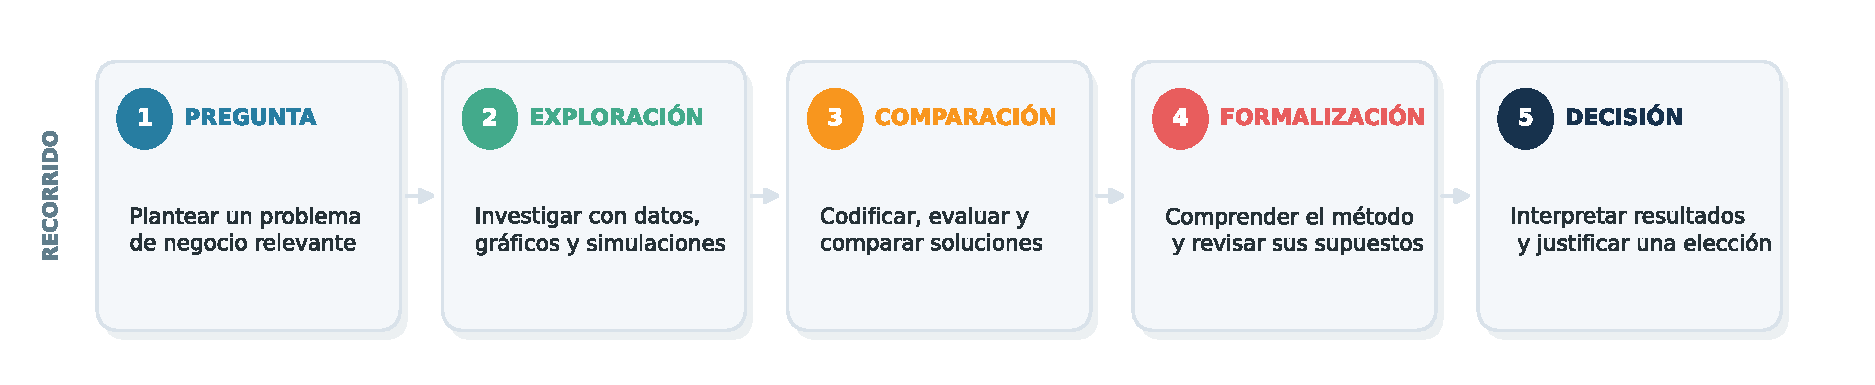
\includegraphics[width=1\linewidth,height=\textheight,keepaspectratio]{presentacion_ejercicio_files/mediabag/figures/fig_metodologia.pdf}

Las sesiones prácticas desarrollan los contenidos de la teoría y
producen evidencias de aprendizaje durante todo el cuatrimestre.

\note{{[}\ldots{]} que se resume en cinco pasos: pregunta relevante,
exploración de los datos, comparación de métodos, formalización y
decisión.

Es un recorrido que va de la narrativa a lo visual, de lo visual a la
implementación y del código a lo formal.

El orden es deliberado: la formalización llega cuando el estudiante ha
visto el problema, ha manipulado los datos y ha comparado modelos. Las
sesiones prácticas desarrollan así los contenidos de la teoría y
producen evidencias de aprendizaje durante todo el cuatrimestre.}
\end{frame}

\begin{frame}[fragile]{Recursos didácticos}
\phantomsection\label{recursos-diduxe1cticos}
~

\begin{longtable}[]{@{}
  >{\raggedright\arraybackslash}p{(\linewidth - 4\tabcolsep) * \real{0.2308}}
  >{\raggedright\arraybackslash}p{(\linewidth - 4\tabcolsep) * \real{0.3846}}
  >{\raggedright\arraybackslash}p{(\linewidth - 4\tabcolsep) * \real{0.3846}}@{}}
\toprule\noalign{}
\begin{minipage}[b]{\linewidth}\raggedright
Tipo de recurso
\end{minipage} & \begin{minipage}[b]{\linewidth}\raggedright
Elementos
\end{minipage} & \begin{minipage}[b]{\linewidth}\raggedright
Uso
\end{minipage} \\
\midrule\noalign{}
\endhead
\bottomrule\noalign{}
\endlastfoot
\textbf{Software y bibliotecas} & \texttt{Python},
\texttt{scikit-learn}, \texttt{Keras} y \texttt{DoubleML} &
Implementación y comparación de métodos \\ \lightrowrule
\textbf{Entornos de trabajo} & \texttt{Jupyter}, Google Colab, IDE y
entorno \texttt{conda} versionado & Desarrollo, acceso y ejecución
reproducible \\ \lightrowrule
\textbf{Materiales expositivos} & Notas, presentaciones y ejemplos de
código & Introducción y explicación de los contenidos \\ \lightrowrule
\textbf{Materiales prácticos} & Notebooks guiados, ejercicios y datos
reales & Aplicación progresiva de los métodos \\ \lightrowrule
\textbf{Recursos interactivos} & Simulaciones y visualizaciones &
Exploración de concepts: p.e. sesgo, incertidumbre y variabilidad, o
entrenamiento de redes neuronales \\ \lightrowrule
\textbf{Recursos para la evaluación} & Cuestionarios breves y
actividades de autoevaluación & Seguimiento y retroalimentación \\ \lightrowrule
\textbf{Recursos para la reproducibilidad} & Repositorio de la
asignatura y plantillas & Organización, documentación y reutilización \\ \lightrowrule
\textbf{Bibliografía} & James et al., \textbf{ISLP} (2023) + lecturas
específicas y documentación de bibliotecas & Fundamentación y ampliación
de contenidos \\ \lightrowrule
\end{longtable}

\note{¿Qué recursos didácticos apoyan el aprendizaje? Los agrupo en ocho
tipos: software y entornos de trabajo, materiales expositivos y
prácticos, recursos interactivos, recursos para la evaluación y para la
reproducibilidad, y bibliografía.

Una de las decisiones más relevantes del curso es la elección del
software y entorno. A pesar de que el alumnado llega con una formación
amplia en \texttt{R}, la asignatura se desarrolla en \texttt{Python},
utilizando las librerias \texttt{scikit-learn}, \texttt{Keras} y
\texttt{DoubleML}. Las razones son tanto profesionales como docentes:

\begin{enumerate}
\tightlist
\item
  \texttt{Python} ofrece librerías de referencia para métodos
  avanzados,\\
\item
  es una herramienta ampliamente utilizada en la industria de datos y
\item
  permite trabajar en la nube a través de Google Colab, sin
  instalaciones locales.
\end{enumerate}

Además, el cambio de lenguaje persigue un objetivo fundamental: que el
alumnado \textbf{aprenda a transferir sus conocimientos y comprenda que
cambia la herramienta, pero no el concepto}.}
\end{frame}

\begin{frame}{Evaluación}
\phantomsection\label{evaluaciuxf3n}
~

\begin{center}
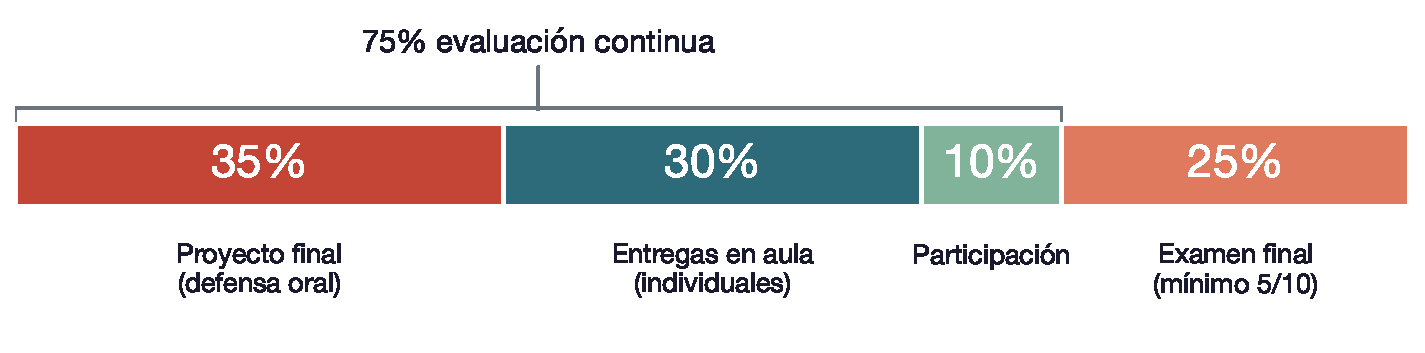
\includegraphics[width=0.5\linewidth,height=\textheight,keepaspectratio]{presentacion_ejercicio_files/mediabag/figures/fig_evaluacion.pdf}
\end{center}

\begin{itemize}
\tightlist
\item
  \textbf{Proyecto (35\%)}: aplicación integrada de los contenidos y
  defensa oral.
\item
  \textbf{Entregas (30\%) y participación (10\%)}: seguimiento del
  trabajo individual durante el curso.
\item
  \textbf{Examen (25\%)}: preguntas teóricas y aplicadas; se exige un
  mínimo de \textbf{5/10}.
\end{itemize}

Los pesos, las rúbricas y las condiciones de recuperación se publican al
inicio del curso.

\note{El último hito en el diseño de la asignatura es la evaluación,
donde, dada su naturaleza, la práctica y la evaluación continua tienen
un peso sustantivo. Dentro de esta destaca el proyecto final con defensa
oral que supone un treinta y cinco por ciento de la nota. Por otro lado
un examen final escrito pondera el veinticinco por ciento de la nota
final.

El diseño responde a la metodología: si el aprendizaje se produce
mayoritariamente en la práctica semanal y a través de un proyecto, la
mayor parte de la nota tiene que salir de ahí. El examen conserva un
peso suficiente para comprobar que cada estudiante domina
individualmente los conceptos, y fijar un mínimo de 5 evita que una
buena nota de proyecto compense la falta de base.}

\gdef\roadmapcontent{{\scriptsize \mbox{\color{black!40}Parte 1 · Currículum}\quad \mbox{\color{mDarkTeal}\bfseries Parte 2 · Propuesta docente}\quad \mbox{\color{black!40}Parte 3 · Propuesta investigadora: Creative collaborations}\par}
\vspace{0.8em}
{\large \mbox{\color{black!40}Técnicas avanzadas de predicción}~· \mbox{\color{mDarkTeal}\bfseries Proyecto final}~· \mbox{\color{black!40}Tema 7. Predicción y efectos causales}\par}}
\end{frame}

\section{Proyecto final}\label{proyecto-final}

\begin{frame}[fragile]{Proyecto del cuatrimestre}
\phantomsection\label{proyecto-del-cuatrimestre}
~

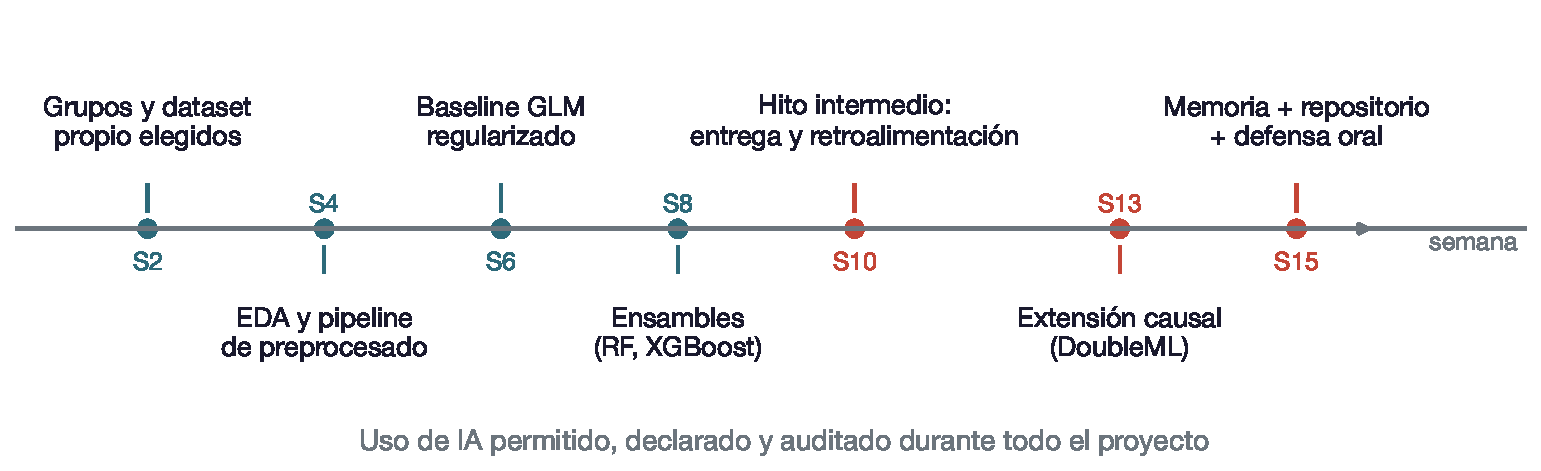
\includegraphics[width=0.88\linewidth,height=\textheight,keepaspectratio]{presentacion_ejercicio_files/mediabag/figures/fig_timeline_proyecto.pdf}

\begin{itemize}
\tightlist
\item
  Grupos de 3--4 alumnos, dataset y problema propios elegidos en la
  semana 2; cada entrega se basa en el contenido desarrollado durante
  esas semanas
\item
  El hito de la S13 permite formular una pregunta causal sobre los
  propios datos y responderla con \texttt{DoubleML} (o justificar por
  qué los supuestos no lo permiten)
\item
  Entrega final: \textbf{repositorio reproducible + memoria + defensa
  oral}
\end{itemize}

\note{¿Cómo se desarrolla el proyecto en grupos? Este se organiza a lo
largo de una serie de entregas parciales durante todo el cuatrimestre.

Los grupos, de tres o cuatro estudiantes, eligen en la semana dos su
propio conjunto de datos y el problema al que responde. A partir de ahí
el trabajo evoluciona en paralelo con las prácticas: hacia la mitad del
cuatrimestre hay una entrega con retroalimentación y en la semana trece,
como aspecto opcional, se puede formular una extensión causal al modelo
predictivo. La entrega de la memoria, el respositorio y la presentación
tienen lugar en la semana quince.

Es importante señalar que durante todo el recorrido el uso de
inteligencia artificial está permitido, declarado y auditado. La entrega
final, repositorio reproducible, memoria y defensa oral, se califica con
una rúbrica{[}\ldots{]}}
\end{frame}

\begin{frame}[shrink]{Rúbrica del proyecto}
\phantomsection\label{ruxfabrica-del-proyecto}
~

\begin{longtable}[]{@{}
  >{\raggedright\arraybackslash}p{(\linewidth - 8\tabcolsep) * \real{0.2000}}
  >{\raggedright\arraybackslash}p{(\linewidth - 8\tabcolsep) * \real{0.2000}}
  >{\raggedright\arraybackslash}p{(\linewidth - 8\tabcolsep) * \real{0.2000}}
  >{\raggedright\arraybackslash}p{(\linewidth - 8\tabcolsep) * \real{0.2000}}
  >{\raggedright\arraybackslash}p{(\linewidth - 8\tabcolsep) * \real{0.2000}}@{}}
\toprule\noalign{}
\begin{minipage}[b]{\linewidth}\raggedright
\textbf{Dimensión (peso)}
\end{minipage} & \begin{minipage}[b]{\linewidth}\raggedright
\textbf{Qué se evalúa}
\end{minipage} & \begin{minipage}[b]{\linewidth}\raggedright
\textbf{Excelente (9--10)}
\end{minipage} & \begin{minipage}[b]{\linewidth}\raggedright
\textbf{Apto (5--6)}
\end{minipage} & \begin{minipage}[b]{\linewidth}\raggedright
\textbf{No apto}
\end{minipage} \\
\midrule\noalign{}
\endhead
\bottomrule\noalign{}
\endlastfoot
\textbf{Formulación y datos (10\%)} & Pregunta relevantes, dataset, EDA
& pregunta orientada a toma decisiones susceptible de respuesta
empírica; limitaciones de los datos discutidas & Pregunta clara, EDA
correcto & Dataset sin justificar; pregunta ambigua; EDA ausente \\ \lightrowrule
\textbf{Proyecto reproducible (20\%)} & Repositorio, entorno, ejecución
(\emph{pipeline}) & Reproduce todo desde datos crudos, entorno
versionado & Reproducible con intervención menor documentada & No
reproduce; preprocesado fuera del pipeline (fuga) \\ \lightrowrule
\textbf{Modelización (25\%)} & Modelo base → ensambles → SVM → DL;
comparación & Comparación honesta en test común; selección justificada &
\(\geq\) 3 familias comparadas correctamente; métricas incompletas & Sin
modelo base; métricas elegidas a posteriori \\ \lightrowrule
\textbf{Interpretación y comunicación (15\%)} & Memoria, figuras,
lectura de resultados & Resultados traducidos a decisión de negocio;
incorpora incertidumbre & Interpretación correcta de métricas y efectos
& Lectura mecánica o errónea de las salidas \\ \lightrowrule
\textbf{Defensa oral individual (30\%)} & 10' grupo + preguntas
individuales & Cada miembro explica y modifica en vivo cualquier parte
del código & Cada miembro explica las partes que firmó & Un miembro no
sabe explicar código propio \\ \lightrowrule
\end{longtable}

\note{{[}\ldots{]} que contempla cinco dimensiones con su peso, lo que
se observa en cada una y los descriptores de tres niveles: excelente,
apto y no apto. Es importante mencionar que la defensa oral individual
pesa un treinta por ciento de la nota del proyecto.

La última pieza del proyecto es la política de uso de inteligencia
artificial.}
\end{frame}

\begin{frame}[shrink]{Uso de inteligencia artificial}
\phantomsection\label{uso-de-inteligencia-artificial}
~

\begin{columns}[T]
\begin{column}{0.3\linewidth}
\begin{center}\rule{0.5\linewidth}{0.5pt}\end{center}

\textbf{Tres verificaciones (que la IA no suplanta)}

\begin{center}\rule{0.5\linewidth}{0.5pt}\end{center}

\begin{itemize}
\tightlist
\item
  \textbf{Defensa oral individual} con modificación de código en vivo
\item
  \textbf{10\% de participación en aula} (presencialidad verificada)
\item
  \textbf{Examen presencial} (25\%) con mínimo de 5/10
\end{itemize}

\begin{center}\rule{0.5\linewidth}{0.5pt}\end{center}
\end{column}

\begin{column}{0.05\linewidth}
\end{column}

\begin{column}{0.65\linewidth}
~

\textbf{Política de IA: permitida, declarada, auditada}

\begin{itemize}
\tightlist
\item
  Uso libre de asistentes para código, depuración y redacción
  (favoreciendo uso crítico y responsable)
\item
  \textbf{Obligatorio:} el registro completo de prompts se entrega como
  apéndice del proyecto y de las entregas relevantes
\item
  Evaluado sobre los prompts: el registro se cruza con el código y la
  memoria buscando coherencia prompts \(\leftrightarrow\) trabajo; se
  valora la transparencia. Alerta si resultado excede lo que el registro
  explica
\end{itemize}
\end{column}
\end{columns}

\note{En un trabajo que exige, entre otras cosas, programar es del todo
irreal tratar de evitar que el alumnado se apoye en herramientas de
inteligencia artificial. La respuesta debe ser integrar y supervisar su
uso, no prohibirlo o ignorarlo.

Los estudiantes pueden usar libremente asistentes o agentes para
programar, depurar y redactar, con un uso crítico y responsable. A
cambio hay una obligación: el registro completo de los prompts, no una
selección, se entrega como apéndice del proyecto y de las entregas
relevantes.

Y ese registro se evalúa: se cruza con el código y con la memoria
buscando coherencia entre el proceso declarado y el trabajo entregado.
La transparencia se valora positivamente; cuando el resultado no puede
explicarse suficientemente a partir del proceso documentado, será
necesario examinarlo con mayor profundidad.

Además, hay tres verificaciones que la inteligencia artificial no
sustituye: la defensa oral individual, la participación en el aula, que
exige presencialidad, y el examen escrito.}

\gdef\roadmapcontent{{\scriptsize \mbox{\color{black!40}Parte 1 · Currículum}\quad \mbox{\color{mDarkTeal}\bfseries Parte 2 · Propuesta docente}\quad \mbox{\color{black!40}Parte 3 · Propuesta investigadora: Creative collaborations}\par}
\vspace{0.8em}
{\large \mbox{\color{black!40}Técnicas avanzadas de predicción}~· \mbox{\color{black!40}Proyecto final}~· \mbox{\color{mDarkTeal}\bfseries Tema 7. Predicción y efectos causales}\par}}
\end{frame}

\section{Tema 7. Predicción y efectos
causales}\label{tema-7.-predicciuxf3n-y-efectos-causales}

\note{Finalizo la propuesta docente presentando brevemente el Tema 7,
que empieza con una decisión de negocio: los alumnos están
familiarizados con la problemática que el abandono de clientes supone
para las empresas. Un problema que conocen desde un marco predictivo. En
este tema partimos de la modelización del \emph{riesgo de abandono} para
ir un paso más allá y estimar parámetros estructurales.}

\begin{frame}[shrink]{Riesgo de abandono y estrategia de retención de
clientes}
\phantomsection\label{riesgo-de-abandono-y-estrategia-de-retenciuxf3n-de-clientes}
~

\begin{columns}[T]
\begin{column}{0.3\linewidth}
\begin{center}\rule{0.5\linewidth}{0.5pt}\end{center}

\textbf{Decisión de negocio}: estimación del riesgo de abandono
(\emph{churn}) y estrategia retención de clientes. Analizamos dos reglas
de priorización

\begin{itemize}
\tightlist
\item
  \textbf{RISK:} actuar sobre quienes tienen mayor probabilidad de
  abandono.\\
\item
  \textbf{LIFT:} actuar sobre quienes la intervención produce una mayor
  reducción de la probabilidad de abandono (sensibilidad a la
  intervención).
\end{itemize}

\begin{center}\rule{0.5\linewidth}{0.5pt}\end{center}

La predicción del riesgo de abandono no responde por sí sola a la
cuestión de gestión \textbf{qué clientes deberían ser objeto de una
campaña}. Esta decisión requiere estimar el efecto causal de la
intervención.

\begin{center}\rule{0.5\linewidth}{0.5pt}\end{center}
\end{column}

\begin{column}{0.05\linewidth}
\end{column}

\begin{column}{0.65\linewidth}
\begin{tcolorbox}[enhanced jigsaw, colback=white, left=2mm, bottomrule=.15mm, toptitle=1mm, title={Experimentos aleatorios controlados: el patrón de referencia}, coltitle=black, colbacktitle=quarto-callout-note-color!10!white, breakable, titlerule=0mm, leftrule=.75mm, colframe=quarto-callout-note-color-frame, rightrule=.15mm, opacityback=0, bottomtitle=1mm, arc=.35mm, toprule=.15mm, opacitybacktitle=0.6]

Ascarza (2018). ``Retention Futility: Targeting High-Risk Customers
Might Be Ineffective'', \emph{Journal of Marketing Research}, 55(1),
80--98. DOI: 10.1509/jmr.16.0163.

Un operador de telefonía móvil de prepago de Oriente Medio asignó al
azar a 12.137 clientes que habían recargado entre una y cuatro semanas
antes y no habían realizado llamadas durante la última semana. El grupo
tratado recibió un SMS con crédito adicional si recargaba una cantidad
determinada en los tres días siguientes. Se observó si la línea seguía
activa 30 días después.

Con los resultados derivados de los datos experimentales se estima qué
impacto tendría una campaña de retención sobre un subconjunto de los
clientes (40\%) usando reglas de priorización alternativas: RISK o LIFT.

\end{tcolorbox}

~

\begin{longtable}[]{@{}
  >{\raggedright\arraybackslash}p{(\linewidth - 4\tabcolsep) * \real{0.3913}}
  >{\raggedright\arraybackslash}p{(\linewidth - 4\tabcolsep) * \real{0.3913}}
  >{\centering\arraybackslash}p{(\linewidth - 4\tabcolsep) * \real{0.2174}}@{}}
\toprule\noalign{}
\begin{minipage}[b]{\linewidth}\raggedright
Criterio de selección
\end{minipage} & \begin{minipage}[b]{\linewidth}\raggedright
Pregunta que responde
\end{minipage} & \begin{minipage}[b]{\linewidth}\centering
Efecto
\end{minipage} \\
\midrule\noalign{}
\endhead
\bottomrule\noalign{}
\endlastfoot
Seleccionar el 40\% de los clientes con mayor \textbf{riesgo} (problema
predictivo) & ¿Quién es más probable que abandone? & \textbf{-1.9
puntos} \\ \lightrowrule
Seleccionar el 40\% de los clientes con mayor \textbf{sensibilidad a la
intervención} (problema inferencia causal) & ¿En quién reduce la campaña
el abandono? & \textbf{-6,0 puntos} \\ \lightrowrule
\end{longtable}

La diferencia entre ambos criterios fue de \textbf{4,1 puntos
porcentuales}.
\end{column}
\end{columns}

\note{Empezamos con una pregunta práctica: ante el riesgo de abandono,
¿a qué clientes dirigir una campaña de retención? Caben dos reglas. La
primera, RISK, actúa sobre quienes tienen mayor probabilidad de
abandonar: un problema predictivo. La segunda, LIFT, actúa sobre
aquellos en quienes la intervención más reduce ese riesgo: un problema
de inferencia causal, porque exige saber cómo responderían ante una
situación que no observamos.

En el aula lo ilustramos con el experimento de Ascarza (2018). Un
operador de telefonía móvil asignó aleatoriamente a 12.000 clientes
inactivos una oferta de crédito condicionada a una recarga y comprobó,
treinta días después, si la línea seguía activa. Con esos datos, la
autora simula una campaña dirigida al cuarenta por ciento superior de
los clientes según cada regla: seleccionar por sensibilidad a la
intervención reduce más el abandono que seleccionar por riesgo.

El mensaje es claro: la predicción por sí sola no responde a la pregunta
de negocio; para eso hay que estimar el efecto causal.}
\end{frame}

\begin{frame}[shrink]{Aprendizaje automático para la estimación de
efectos causales}
\phantomsection\label{aprendizaje-automuxe1tico-para-la-estimaciuxf3n-de-efectos-causales}
~

\begin{columns}[T]
\begin{column}{0.3\linewidth}
\begin{center}\rule{0.5\linewidth}{0.5pt}\end{center}

\textbf{Objetivo}: estimar el parámetro \(\tau\) para la expresión:
\[y=\tau D+g(X)+\epsilon\]

\begin{center}\rule{0.5\linewidth}{0.5pt}\end{center}

Con \textbf{datos observacionales} \(\to\) posible confusión en \(X\):

\[D= m(X)+\eta\]

\begin{center}\rule{0.5\linewidth}{0.5pt}\end{center}
\end{column}

\begin{column}{0.05\linewidth}
\end{column}

\begin{column}{0.65\linewidth}
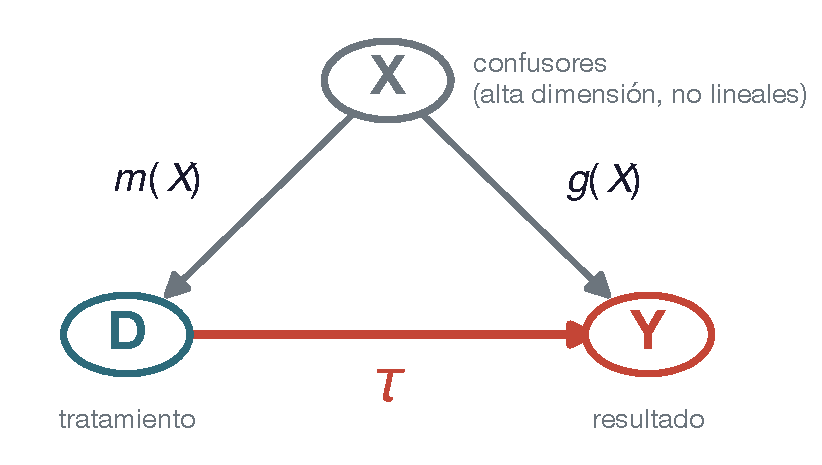
\includegraphics[width=0.72\linewidth,height=\textheight,keepaspectratio]{presentacion_ejercicio_files/mediabag/figures/fig_dag_confusion_sin_ecuacion.pdf}

\textbf{¿Por qué aprendizaje automático?}

\begin{itemize}
\tightlist
\item
  Elevada dimensionalidad de \(X\).
\item
  Datos no tabulares (p.e. texto o imágenes).
\item
  Flexibilidad para aproximar \(g\) y \(m\).
\end{itemize}
\end{column}
\end{columns}

\note{Si nos movemos del contexto al modelo, el objetivo es estimar el
efecto que una intervención \(D\) tiene sobre la respuesta \(y\) (el
parámetro \(\tau\)) asumiendo que y depende a su vez de un conjunto de
variables auxiliares X.

Si trabajamos con datos observacionales debemos, además, considerar la
posibilidad de confusión si la selección al tratamiento se ve afectada
las variables \(X\): incorporamos este proceso a través de la función
\(m\).

El grafo visualiza el mecanismo generador de datos y explicita
\textbf{el objetivo del tema: la incorporación técnicas de aprendizaje
máquina para la estimación de tau}

ML, ¿por qué? Tres motivos: elevada dimensionalidad de X, el uso de
datos no tabulares (texto o imágenes) o la complejidad de \(g\) o \(m\)
(no linealidad, interacciones) que podemos aproximar a través de modelos
flexibles sin la necesidad de especificarlos.}
\end{frame}

\begin{frame}[shrink]{De la aplicación \emph{naive} al Double Machine
Learning}
\phantomsection\label{de-la-aplicaciuxf3n-naive-al-double-machine-learning}
~

\begin{columns}[T]
\begin{column}{0.38\linewidth}
\begin{center}\rule{0.5\linewidth}{0.5pt}\end{center}

\textbf{Estimación \emph{naive} del modelo parcialmente lineal
\(y=\tau D + g(X)+ \epsilon\)}

\begin{enumerate}
\tightlist
\item
  Aprender \(\hat{g}\) y residualizar la respuesta:
  \(\tilde{y}=y-\hat{g}(X)\).\\
\item
  Regresión de \(\tilde{y}\) sobre \(D\).
\end{enumerate}

\begin{center}\rule{0.5\linewidth}{0.5pt}\end{center}

\textbf{Double Machine Learning}

\begin{enumerate}
\tightlist
\item
  Aprender \(\hat{g}\), \(\hat{m}\); residualizar respuesta y
  tratamiento con \emph{cross-fitting}: \(\tilde{y}=y-\hat{g}(X)\),
  \(\tilde{D}=D-\hat{m}(X)\).
\item
  Regresión de \(\tilde{y}\) sobre \(\tilde{D}\):
  \(\tilde{y}=\tau\tilde{D}+\epsilon\).
\end{enumerate}

\begin{center}\rule{0.5\linewidth}{0.5pt}\end{center}
\end{column}

\begin{column}{0.04\linewidth}
\end{column}

\begin{column}{0.58\linewidth}
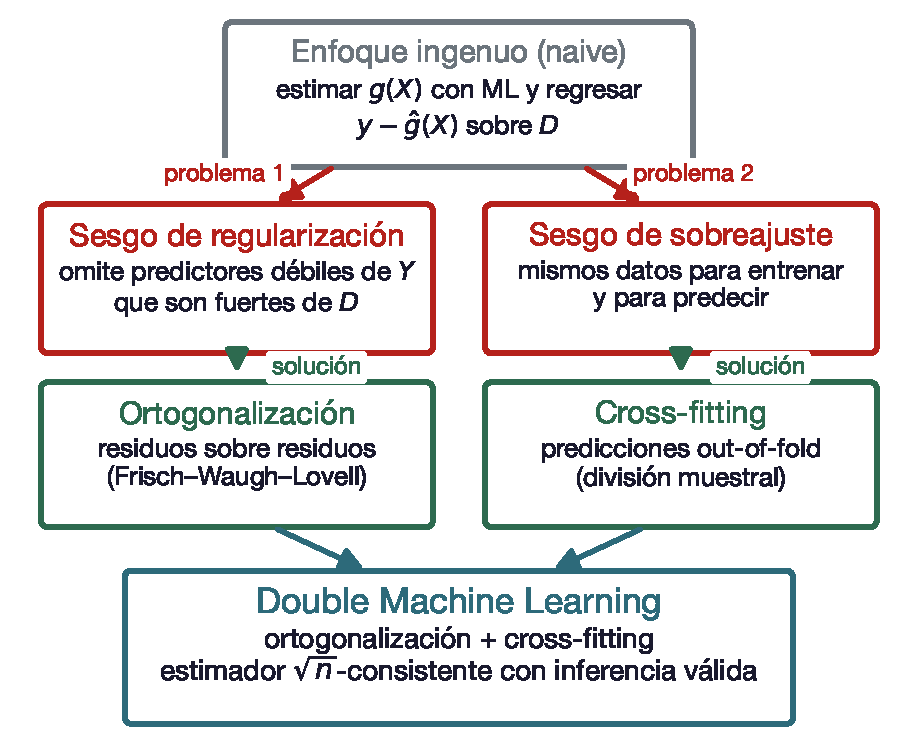
\includegraphics[width=0.8\linewidth,height=\textheight,keepaspectratio]{presentacion_ejercicio_files/mediabag/figures/fig_esquema_dml.pdf}
\end{column}
\end{columns}

\note{La aplicación ingenua del aprendizaje automático al modelo
parcialmente lineal supone aprender un modelo flexible para \(g\),
residualizar la respuesta y regresar ese residuo sobre el tratamiento.
Falla por dos motivos.

El primero es el \textbf{sesgo de regularización}. El modelo selecciona
las variables por su capacidad para predecir \(y\): un control poco
correlacionado con la respuesta pero relevante para explicar \(D\) queda
atenuado o fuera. Es, un \textbf{sesgo de variable omitida}.

El segundo es el \textbf{sesgo por sobreajuste}: si se entrena y se
predice sobre las mismas observaciones, los residuos absorben parte del
efecto causal y la varianza residual del tratamiento se distorsiona.

Double Machine Learning corrige ambos. Corrige el primero, la
ortogonalización residualiza también el tratamiento con la función
auxiliar \(m\). Corrige el segundo, el cross-fitting separa las
observaciones con las que se entrena de aquellas sobre las que se
predice. El resultado es un estimador raíz de \(n\) consistente con
inferencia válida, que los estudiantes implementan con DoubleML como un
estimador en dos etapas.}
\end{frame}

\begin{frame}[fragile,shrink]{Práctica con datos reales}
\phantomsection\label{pruxe1ctica-con-datos-reales}
~

\begin{columns}[T]
\begin{column}{0.3\linewidth}
\textbf{Workflow con \texttt{DoubleML}}

\begin{Shaded}
\begin{Highlighting}[]
\ImportTok{from}\NormalTok{ doubleml }\ImportTok{import}\NormalTok{ DoubleMLData, }\OperatorTok{\textbackslash{}}
\NormalTok{   DoubleMLPLR}
\ImportTok{from}\NormalTok{ sklearn.ensemble }\ImportTok{import} \OperatorTok{\textbackslash{}}
\NormalTok{   RandomForestRegressor}

\NormalTok{datos }\OperatorTok{=}\NormalTok{ DoubleMLData(df, y\_col}\OperatorTok{=}\StringTok{"gasto"}\NormalTok{,}
\NormalTok{                     d\_cols}\OperatorTok{=}\StringTok{"email"}\NormalTok{,}
\NormalTok{                     x\_cols}\OperatorTok{=}\NormalTok{covariables)}

\NormalTok{regresor }\OperatorTok{=}\NormalTok{ RandomForestRegressor()}

\NormalTok{dml }\OperatorTok{=}\NormalTok{ DoubleMLPLR(datos,}
\NormalTok{                  ml\_l}\OperatorTok{=}\NormalTok{regresor,}
\NormalTok{                  ml\_m}\OperatorTok{=}\NormalTok{regresor,}
\NormalTok{                  n\_folds}\OperatorTok{=}\DecValTok{5}\NormalTok{)}
\NormalTok{dml.fit()}
\BuiltInTok{print}\NormalTok{(dml.summary)}
\NormalTok{dml.sensitivity\_analysis()}
\end{Highlighting}
\end{Shaded}
\end{column}

\begin{column}{0.05\linewidth}
\end{column}

\begin{column}{0.65\linewidth}
\textbf{Decisión: ¿a quién enviar la campaña?}

\begin{itemize}
\tightlist
\item
  Los
  \href{https://www.minethatdata.com/Kevin_Hillstrom_MineThatData_E-MailAnalytics_DataMiningChallenge_2008.03.20.csv}{datos
  públicos de Hillstrom} incluyen 64.000 clientes asignados al azar a
  tres grupos: email de productos de hombre, email de productos de mujer
  y control sin email. Durante dos semanas se observan visitas, compras
  y gasto.
\item
  Se estima el efecto promedio de la intervención y se comparan dos
  reglas de priorización: selección por probabilidad de respuesta
  positiva o por efecto estimado de la campaña.
\item
  En una etapa final se introduce selección observacional y valida
  \texttt{DoubleML} frente al resultado experimental.
\end{itemize}

\textbf{Salida del workflow:} los modelos de primera etapa se evalúan
con validación cruzada; \texttt{dml} devuelve el efecto estimado, su
intervalo de confianza y la sensibilidad a confusión residual.
\end{column}
\end{columns}

\note{Los alumnos aplican la teoría a la evaluación de una campaña de
emailing con los datos experimentales de Hillstrom. Siguiendo un flujo
de trabajo ya conocido de los temas predictivos, estiman el efecto
promedio, comparan reglas de priorización y, tras introducir selección
observacional, evalúan si DoubleML recupera el efecto conocido.

La evaluación no exige demostraciones ni desarrollos formales. Se evalúa
la capacidad para distinguir entre predicción de intervención,
identificar sesgos, aplicar ortogonalización y cross-fitting, realizar
inferencia y valorar los supuestos y por tanto límites del análisis.}
\end{frame}

\begin{frame}
\partdividercontent{Parte 3 de 3}{Propuesta investigadora: \emph{Creative collaborations}}{{\scriptsize \mbox{\color{black!40}Parte 1 · Currículum}\quad \mbox{\color{black!40}Parte 2 · Propuesta docente}\quad \mbox{\color{mDarkTeal}\bfseries Parte 3 · Propuesta investigadora: Creative collaborations}\par}}

\note{Cierro el ejercicio presentando la propuesta de investigación
\emph{Creative Collaborations}, cuyo objeto es el análisis de los
factores asociados a la formación de colaboraciones en la producción
cultural.}
\end{frame}

\begin{frame}{De qué trata esta investigación}
\phantomsection\label{de-quuxe9-trata-esta-investigaciuxf3n}
~

\begin{longtable}[]{@{}
  >{\raggedright\arraybackslash}p{(\linewidth - 2\tabcolsep) * \real{0.2200}}
  >{\raggedright\arraybackslash}p{(\linewidth - 2\tabcolsep) * \real{0.7800}}@{}}
\toprule\noalign{}
\endhead
\bottomrule\noalign{}
\endlastfoot
\textbf{Colaborar} & Dos artistas graban juntos una canción, el fenómeno
\emph{feat.}: \textbf{Bad Bunny y J Balvin}, \textbf{Taylor Swift y
Kendrick Lamar}. Hoy es una práctica frecuente. \\ \lightrowrule
\textbf{Elección} & Cada artista podría colaborar con cientos de otros y
solo lo hace con unos pocos. ¿Qué distingue a los pares que llegan a
trabajar juntos? \\ \lightrowrule
\textbf{Proximidad estética} & En redes sociales el público describe a
cada artista con etiquetas (palabras): géneros, estilos, estados de
ánimo. \textbf{Bad Bunny y J Balvin} son etiquetados con un vocabulario
similar (\emph{cercanos}). \textbf{Taylor Swift y kendrick Lamar} apenas
comparten (\emph{distantes}). \\ \lightrowrule
\textbf{La hipótesis} & Estar cerca facilita el encaje: Bad Bunny y J
Balvin han grabado juntos en varias ocasiones. Pero también colaboran
artistas lejanos: Taylor Swift y Kendrick Lamar. ¿Hay un punto a partir
del cual parecerse más ya no suma, o incluso resta? \\ \lightrowrule
\end{longtable}

\begin{tcolorbox}[enhanced jigsaw, colback=white, left=2mm, bottomrule=.15mm, toptitle=1mm, title={Y no solo la dimensión estética}, coltitle=black, colbacktitle=quarto-callout-note-color!10!white, breakable, titlerule=0mm, leftrule=.75mm, colframe=quarto-callout-note-color-frame, rightrule=.15mm, opacityback=0, bottomtitle=1mm, arc=.35mm, toprule=.15mm, opacitybacktitle=0.6]

Contactos previos en la red de colaboraciones, escena cultural e
institucional y trayectoria de cada artista. Datos: quién colabora con
quién en las listas globales de Spotify, 2013--2025.

\end{tcolorbox}

\note{Resumo la propuesta en cuatro ideas.

\begin{enumerate}
\tightlist
\item
  Colaborar es grabar juntos una canción, como Bad Bunny y J Balvin o
  Taylor Swift y Kendrick Lamar.\\
\item
  La colaboración implica una decisión: cada artista podría colaborar
  con muchos y solo lo hace con pocos; la pregunta es qué distingue a
  los pares que llegan a trabajar juntos.\\
\item
  Para responderla cada artista se ubica en un espacio construido a
  partir de las etiquetas que su público publica en redes. Bad Bunny y J
  Balvin tienen un vocabulario casi idéntico (proximidad); Bad Bunny y
  Ed Sheeran apenas comparten palabras (distancia).
\item
  La hipótesis central es que estar cerca ayuda: de hecho Bad Bunny y J
  Balvin han grabado juntos varias veces. Pero, ¿y si se está demasiado
  cerca? ¿Hay un punto en que parecerse más ya no aporta?
\end{enumerate}

En la explicación entra además la red de contactos, trayectoria y otros
atributos.}

\gdef\roadmapcontent{{\scriptsize \mbox{\color{black!40}Parte 1 · Currículum}\quad \mbox{\color{black!40}Parte 2 · Propuesta docente}\quad \mbox{\color{mDarkTeal}\bfseries Parte 3 · Propuesta investigadora: Creative collaborations}\par}
\vspace{0.8em}
{\large \mbox{\color{mDarkTeal}\bfseries Motivación y pregunta económica}~· \mbox{\color{black!40}Datos y diseño}~· \mbox{\color{black!40}Resultados}~· \mbox{\color{black!40}Conclusiones}\par}}
\end{frame}

\section{Motivación y pregunta
económica}\label{motivaciuxf3n-y-pregunta-econuxf3mica}

\note{La presentación se estructura en cuatro partes.

\begin{itemize}
\item
  Comienzo por la motivación, la definición del problema económico y por
  una hipótesis sobre afinidad en un espacio estético.
\item
  Después presento medición y diseño.
\item
  Los resultados combinan inferencia y evaluación predictiva, seguidas
  de sus comprobaciones.
\item
  Cierro con la aportación, sus límites y las preguntas que abre.
\end{itemize}}

\begin{frame}{La colaboración en la industria de la música}
\phantomsection\label{la-colaboraciuxf3n-en-la-industria-de-la-muxfasica}
~

\begin{figure}[H]

{\centering 
\includegraphics[width=0.92\linewidth,height=\textheight,keepaspectratio]{presentacion_ejercicio_files/mediabag/figures/fig_billboard_trend.pdf}

}

\caption{Proporción de colaboraciones en el Billboard Hot 100 por año y
tramo de la lista, 1970-2025, con ajuste local.}

\end{figure}%

\note{La figura muestra la evolución del porcentaje de colaboraciones en
listas anuales del Billboard 100 (además de en subtramos de la misma) y
sirve como punto de partida para ilustrar la pregunta.

A comienzos de los setenta, menos del 3\% de las entradas anuales del
Billboard correspondían a colaboraciones. Entre 2016 y 2020 esa tasa se
sitúa en torno al 40\%: la colaboración ha pasado de ser una anomalía
entre los éxitos comerciales a la práctica habitual. La evolución
sugiere un cambio estructural que emerge en paralelo a la digitalización
de la música y se asienta con la implantación de un modelo de negocio
basado en el acceso, y no en la propiedad: el streaming.

El interés económico de la pregunta de investigación radica en el
análisis de los incentivos en la selección de colaboradores en
industrias culturales. Colaborar permite combinar temporalmente
capacidades y recursos, identidades estéticas, reputación y acceso a
públicos.}
\end{frame}

\begin{frame}[shrink]{Marco conceptual}
\phantomsection\label{marco-conceptual}
~

\begin{longtable}[]{@{}
  >{\raggedright\arraybackslash}p{(\linewidth - 4\tabcolsep) * \real{0.2200}}
  >{\raggedright\arraybackslash}p{(\linewidth - 4\tabcolsep) * \real{0.4800}}
  >{\raggedright\arraybackslash}p{(\linewidth - 4\tabcolsep) * \real{0.3000}}@{}}
\toprule\noalign{}
\begin{minipage}[b]{\linewidth}\raggedright
Pregunta
\end{minipage} & \begin{minipage}[b]{\linewidth}\raggedright
Qué encuentra la literatura
\end{minipage} & \begin{minipage}[b]{\linewidth}\raggedright
Referencias
\end{minipage} \\
\midrule\noalign{}
\endhead
\bottomrule\noalign{}
\endlastfoot
¿Beneficios de colaborar? & Los \emph{featurings} elevan la demanda de
\emph{streaming}; los duetos sobreviven más en las listas & McKenzie et
al.~(2021); Kaimann et al.~(2021) \\ \lightrowrule
¿Qué explica la formación de vínculos? & Mecanismos asortativos,
relacionales y de proximidad geográfica e institucional operan a la vez;
los lazos previos generan información, visibilidad y oportunidades para
nuevos vínculos & Rivera, Soderstrom y Uzzi (2010); Gulati y Gargiulo
(1999); Powell et al.~(2005) \\ \lightrowrule
¿Similares o potencialmente complementarios? & Recursos similares
facilitan coordinación y aprendizaje; los distintos aportan novedad si
emerge complementariedad; el óptimo interior es una hipótesis extendida
en alianzas, innovación y equipos científicos & Mitsuhashi y Greve
(2009); Jones (2009); Nooteboom et al.~(2007); Uzzi et al.~(2013); Smith
et al.~(2021) \\ \lightrowrule
¿Cómo se traduce en la música? & La diferenciación óptima favorece el
éxito; la distancia entre géneros permite potencialmente ampliar la
demanda; la evidencia es sobre los resultados de las colaboraciones;
pero ¿formación? & Askin y Mauskapf (2017); Ordanini, Nunes y Nanni
(2018) \\ \lightrowrule
\end{longtable}

\note{La revisión de la literatura conecta la economía de la cultura con
la formación de equipos y redes, en un campo en el que convergen dos
líneas de investigación.

\begin{enumerate}
\item
  La primera estudia los resultados de las colaboraciones. En música la
  evidencia es clara: las colaboraciones elevan la demanda de
  \emph{streaming} y alargan la supervivencia en listas.
\item
  La segunda estudia la formación de vínculos, con tres familias de
  mecanismos: similitud, conectividad por posición en la red, y
  proximidad geográfica e institucional.
\item
  Un tema recurrente en literatura es la existencia de una distancia
  óptima entre los miembros de una colaboración. Parecerse puede
  facilitar coordinación y compatibilidad; por otro lado la
  diferenciación puede aportar novedad o permitir complementariedades.
\item
  En la industria de la música se ha estudiado sobre todo el éxito de
  las colaboraciones ya realizadas. La evidencia sobre formación es más
  limitada y se concentran en escenas o géneros concretos y,
  metodológicamente, se recurre al muestreo de negativos. Este es el
  principal hueco que se cubre en este papel.
\end{enumerate}}
\end{frame}

\begin{frame}{Contribución: medición y contraste de la afinidad
estética}
\phantomsection\label{contribuciuxf3n-mediciuxf3n-y-contraste-de-la-afinidad-estuxe9tica}
~

\begin{itemize}
\tightlist
\item
  \textbf{Selección de colaboradores}: primeras colaboraciones frente al
  conjunto completo de pares elegibles.
\item
  \textbf{Medición}: perfiles de etiquetas de audiencia asociados a
  lanzamientos anteriores a cada año.
\item
  \textbf{Contraste de forma}: se contrasta un óptimo interior con
  especificaciones flexibles y una prueba prespecificada de reversión de
  signo.
\item
  \textbf{Validación}: inferencia con dependencia diádica, sensibilidad
  y evaluación temporal de la ordenación.
\end{itemize}

\note{La contribución \textbf{combina una pregunta sobre formación de
colaboraciones en industrias culturales con un diseño de la
investigación que permite contrastarla a escala amplia}. El conjunto de
riesgo incluye todos los pares elegibles: así, las colaboraciones
realizadas se comparan con oportunidades definidas de forma explícita.

Además, la identidad estética se representa usando un enfoque basado en
procesamiento del lenguaje natural de las etiquetas generadas por
usuarios en dos redes sociales de música.

La forma de la asociación entre similitud estética y formación de
colaboraciones se contrasta: se parte de una especificación cuadrática
que resume una asociación cóncava y posteriormente se comprueba si los
datos apoyan el tramo decendente tras el óptimo interior.

Finalmente, la inferencia incorpora dependencia entre pares que
comparten artista y la evaluación predictiva se usa para analizar la
asociación que los diferentes bloques de variables capturan fuera de
muestra.}

\gdef\roadmapcontent{{\scriptsize \mbox{\color{black!40}Parte 1 · Currículum}\quad \mbox{\color{black!40}Parte 2 · Propuesta docente}\quad \mbox{\color{mDarkTeal}\bfseries Parte 3 · Propuesta investigadora: Creative collaborations}\par}
\vspace{0.8em}
{\large \mbox{\color{black!40}Motivación y pregunta económica}~· \mbox{\color{mDarkTeal}\bfseries Datos y diseño}~· \mbox{\color{black!40}Resultados}~· \mbox{\color{black!40}Conclusiones}\par}}
\end{frame}

\section{Datos y diseño}\label{datos-y-diseuxf1o}

\begin{frame}[fragile]{Fuentes de datos}
\phantomsection\label{fuentes-de-datos}
~

\begin{columns}[T]
\begin{column}{0.3\linewidth}
\textbf{Cifras básicas}

\begin{longtable}[]{@{}
  >{\raggedright\arraybackslash}p{(\linewidth - 2\tabcolsep) * \real{0.5800}}
  >{\raggedright\arraybackslash}p{(\linewidth - 2\tabcolsep) * \real{0.4200}}@{}}
\toprule\noalign{}
\endhead
\bottomrule\noalign{}
\endlastfoot
Ventana de listas & 2013--2025 \\ \lightrowrule
Pistas × artista & 12.688 \\ \lightrowrule
Artistas en el ámbito & 2.878 \\ \lightrowrule
Con etiquetas fechadas & 2.402 \\ \lightrowrule
\end{longtable}
\end{column}

\begin{column}{0.05\linewidth}
\end{column}

\begin{column}{0.65\linewidth}
\begin{itemize}
\tightlist
\item
  \textbf{\texttt{Spotify}}: listas globales semanales y créditos de
  pista, álbum y artista (metadatos del API).
\item
  \textbf{\texttt{Last.fm} y \texttt{MusicBrainz}}: etiquetas de
  audiencia sobre géneros, estilos y otras percepciones (p.e. estados de
  ánimo).
\item
  \textbf{\texttt{MusicBrainz} y créditos de álbum}: atributos de
  artistas e historial de sellos.
\end{itemize}

\begin{tcolorbox}[enhanced jigsaw, colback=white, left=2mm, bottomrule=.15mm, toptitle=1mm, title={Por qué etiquetas y no géneros de plataforma}, coltitle=black, colbacktitle=quarto-callout-note-color!10!white, breakable, titlerule=0mm, leftrule=.75mm, colframe=quarto-callout-note-color-frame, rightrule=.15mm, opacityback=0, bottomtitle=1mm, arc=.35mm, toprule=.15mm, opacitybacktitle=0.6]

Las etiquetas por lanzamiento cubren el \textbf{83,5\% de los artistas}.
Los géneros de Spotify cubren aproximadamente el \textbf{34\%}.

\end{tcolorbox}
\end{column}
\end{columns}

\note{El trabajo integra tres fuentes. Las listas globales semanales de
Spotify, desde septiembre de 2013 hasta diciembre de 2025, proporcionan
las pistas y los créditos de colaboración. Los metadatos (extraidos del
API web) permiten distinguir al artista principal de los invitados.

Las etiquetas de Last.fm y MusicBrainz aportan una descripción de la
identidad estética desde la audiencia. Cubren el 83,5\% de los artistas
del ámbito inicial pero conviene señalar que medidas alternativas, p.e.
los géneros del API de Spotify, tienen una menor cobertura,
aproximadamente un tercio, y proporciona una lista editorial
seleccionada.

En tercer lugar, los metadatos de MusicBrainz añaden atributos como tipo
de artista, país registrado, año del primer lanzamiento o historial de
sellos (construido con los créditos de álbum observados hasta el año
anterior).

¿Cómo convertir etiquetas textuales de artistas en una medida numérica
comparable de su posición estética? Se propone a continuación una
aproximación novedosa para abordar este problema.}
\end{frame}

\begin{frame}{Proximidad estética}
\phantomsection\label{proximidad-estuxe9tica}
~

\begin{columns}[T]
\begin{column}{0.3\linewidth}
\begin{center}\rule{0.5\linewidth}{0.5pt}\end{center}

\begin{itemize}
\tightlist
\item
  Cada artista es un vector de etiquetas
\item
  La proximidad es la similitud coseno entre vectores
\item
  Cobertura de pares: 93\% de pares con similitud observada en 2015;
  67\% en 2024
\end{itemize}

\begin{center}\rule{0.5\linewidth}{0.5pt}\end{center}
\end{column}

\begin{column}{0.05\linewidth}
\end{column}

\begin{column}{0.65\linewidth}
\begin{center}
\pandocbounded{
\includegraphics[keepaspectratio]{presentacion_ejercicio_files/mediabag/figures/fig_tag_vectors.pdf}}
\end{center}
\end{column}
\end{columns}

\note{Cada artista se representa mediante un vector de etiquetas de
forma que \textbf{su perfil en el año t acumula las etiquetas asociadas
a lanzamientos anteriores a t}.

Dos artistas se comparan por la dirección en la que apuntan sus
vectores, que se articula a través del coseno de ambos (medida
denominada similitud del coseno): cuanto más vocabulario comparten,
mayor es su afinidad en el espacio de etiquetas de usuarios.

La figura muestra una proyección ilustrativa en dos dimensiones, aunque
las similitudes son reales (calculadas con los vectores completos).\\
- Los usuarios etiquetan a Bad Bunny y J Balvin usando un vocabulario
similar de ahí su proximidad en el espacio de etiquetas (con un coseno
igual a 0,82).\\
- Bad Bunny y Ed Sheeran por contra apenas comparten etiquetas y
muestran una baja similitud (0,07).

Además de la proximidad estética, el trabajo incorpora la proximidad
estructural que emerge de la red de colaboraciones, reflejada en
distancia entre nodos o existencia de vecinos comunes.}
\end{frame}

\begin{frame}{Composición de la red}
\phantomsection\label{composiciuxf3n-de-la-red-1}
~


\includegraphics[width=0.88\linewidth,height=\textheight,keepaspectratio]{presentacion_ejercicio_files/mediabag/figures/fig_network_aimac.pdf}

\note{Visualizamos esta proximidad estructural con la representación del
conjunto de datos relacionales en un grafo. La figura muestra solo el
núcleo de la red acumulada hasta el 2024, el 5\% de artistas con mayor
grado, y ofrece una ilustración descriptiva.

El grafo segmenta una escena latina y otra anglófona, con algunos
artistas que conectan ambas. Esto sugiere la necesidad de separar
afinidad (estética o de otro tipo) de posición en la red. Dos artistas
pueden, por ejemplo, compartir espacio cultural y, sin embargo, tener
oportunidades relacionales distintas.}
\end{frame}

\begin{frame}{Qué cuenta como primera colaboración}
\phantomsection\label{quuxe9-cuenta-como-primera-colaboraciuxf3n}
~

\begin{itemize}
\tightlist
\item
  \textbf{Evento}: primera colaboración principal--invitado en una pista
  que entra en listas.
\item
  \textbf{Formación}: exige ausencia de lazos previos entre ambos
  artistas (también los observados fuera de listas).
\item
  \textbf{Pares invitado--invitado}: no cuentan como evento; tampoco
  como negativos.
\end{itemize}

\note{La definición del evento fija el objeto que vamos a estudiar. En
el trabajo se \textbf{considera una primera colaboración cuando un
artista aparece como principal y otro como invitado en una pista que
entra en listas, siempre que no hubiera un lazo previo entre ambos} (se
miden eventos de formación que responden a decisiones distintas de los
de repetición). Los créditos entre dos invitados de una misma pista no
cuentan como formación principal--invitado, pero tampoco son ceros de
colaboración.}
\end{frame}

\begin{frame}{Diseño: el conjunto de oportunidades}
\phantomsection\label{diseuxf1o-el-conjunto-de-oportunidades}
~

\begin{itemize}
\tightlist
\item
  \textbf{Elegibilidad anual}: ambos artistas debutaron antes de \(t\) y
  publicaron una pista en listas en los tres años anteriores.
\item
  \textbf{Conjunto completo de riesgo}: todos los pares no ordenados
  elegibles para una primera colaboración, sin muestreo de negativos.
\item
  \textbf{Muestra de estimación}: 2.256 artistas, 3.756.411 pares-año
  observados en el periodo 2015--2024.
\item
  \textbf{Sensibilidad}: ventana de cinco años y permanencia sin salida
  tras el debut.
\end{itemize}

\begin{tcolorbox}[enhanced jigsaw, colback=white, left=2mm, bottomrule=.15mm, toptitle=1mm, title={Evento raro}, coltitle=black, colbacktitle=quarto-callout-note-color!10!white, breakable, titlerule=0mm, leftrule=.75mm, colframe=quarto-callout-note-color-frame, rightrule=.15mm, opacityback=0, bottomtitle=1mm, arc=.35mm, toprule=.15mm, opacitybacktitle=0.6]

Se identifican con 1.064 eventos de formación elegibles sobre 3.756.411
pares-año: \textbf{28,3 formaciones por cada 100.000 pares-año de
estimación}.

\end{tcolorbox}

\note{El número total de colaboraciones potenciales no es cualquier
combinación imaginable.

\textbf{La investigación define una oportunidad observable}: los dos
artistas deben haber debutado antes del año analizado y tener un tema
que aparece en listas publicado en una ventana que incluye los tres años
anteriores. Además, el par debe seguir siendo elegible para una primera
colaboración (no han colaborado antes).

La ventana de actividad de tres años reduce la presencia de pares con
oportunidades poco plausibles si bien se compara con una ventana de
cinco años y con una variante sin salida tras el debut en listas.

Se utiliza el conjunto de riesgo completo lo que devuelve una muestra de
estimación con 1.064 eventos sobre 3.756.411 pares-año: aproximadamente
28,3 por cada 100.000. La rareza del evento condiciona la inferencia y
la interpretación predictiva.}

\gdef\roadmapcontent{{\scriptsize \mbox{\color{black!40}Parte 1 · Currículum}\quad \mbox{\color{black!40}Parte 2 · Propuesta docente}\quad \mbox{\color{mDarkTeal}\bfseries Parte 3 · Propuesta investigadora: Creative collaborations}\par}
\vspace{0.8em}
{\large \mbox{\color{black!40}Motivación y pregunta económica}~· \mbox{\color{black!40}Datos y diseño}~· \mbox{\color{mDarkTeal}\bfseries Resultados}~· \mbox{\color{black!40}Conclusiones}\par}
\vspace{0.2em}
\hspace{1.5em}{\normalsize \mbox{\color{mDarkTeal}\bfseries Forma de la asociación}~· \mbox{\color{black!40}Predicción}~· \mbox{\color{black!40}Sensibilidad}\par}}
\end{frame}

\section{Resultados · Forma de la
asociación}\label{resultados-forma-de-la-asociaciuxf3n}

\begin{frame}{Estimación}
\phantomsection\label{estimaciuxf3n}
~

\begin{longtable}[]{@{}
  >{\raggedright\arraybackslash}p{(\linewidth - 4\tabcolsep) * \real{0.2000}}
  >{\raggedright\arraybackslash}p{(\linewidth - 4\tabcolsep) * \real{0.4000}}
  >{\raggedright\arraybackslash}p{(\linewidth - 4\tabcolsep) * \real{0.4000}}@{}}
\toprule\noalign{}
\begin{minipage}[b]{\linewidth}\raggedright
\end{minipage} & \begin{minipage}[b]{\linewidth}\raggedright
\textbf{Logit}
\end{minipage} & \begin{minipage}[b]{\linewidth}\raggedright
\textbf{XGBoost}
\end{minipage} \\
\midrule\noalign{}
\endhead
\bottomrule\noalign{}
\endlastfoot
Objetivo & Forma e inferencia de las asociaciones condicionales &
Referencia flexible para ordenar pares; asociaciones fuera de muestra;
forma similitud estética (no paramétrica) \\ \lightrowrule
Especificación & Red retardada, características del par y efectos de año
& Árboles con interacciones y no linealidades \\ \lightrowrule
Diseño temporal & Inferencia 2015--2024; predicción reestimada hasta
2023 & Entrenamiento hasta 2022, validación 2023 y reajuste hasta
2023 \\ \lightrowrule
Evaluación & Ordenación en 2024 & Ordenación en 2024 \\ \lightrowrule
Incertidumbre & Errores estándar robustos diádicos & Bootstrap de
métricas \\ \lightrowrule
\end{longtable}

~

\begin{tcolorbox}[enhanced jigsaw, colback=white, left=2mm, bottomrule=.15mm, toptitle=1mm, title={¿Por qué no un ERGM?}, coltitle=black, colbacktitle=quarto-callout-note-color!10!white, breakable, titlerule=0mm, leftrule=.75mm, colframe=quarto-callout-note-color-frame, rightrule=.15mm, opacityback=0, bottomtitle=1mm, arc=.35mm, toprule=.15mm, opacitybacktitle=0.6]

\begin{enumerate}
\item
  Escalabilidad: con 2.256 actores y millones de díadas la estimación es
  computacionalmente exigente.
\item
  Objeto probabilístico diferente: distribución conjunta de la red
  (ERGM) frente a probabilidad diádica condicional (logit).
\end{enumerate}

Seguimos enfoque de Almquist y Butts (2014).

\end{tcolorbox}

\note{La formación se modeliza a través de dos modelos de clasificación.

\begin{enumerate}
\item
  El logit estima la probabilidad de formación condicionada a la red del
  año anterior y a las características del par. Incluye efectos de año y
  permite hacer inferencia sobre una forma especificada explícitamente.
  Se estiman errores estándar diádicos de Aronow y Samii que admiten
  dependencia entre pares que comparten un artista.
\item
  XGBoost se utiliza como referencia predictiva flexible que además
  aporta evidencia sobre la forma funcional de la proximidad
  estética-propensión a colaborar (sin asumirla). El número de árboles
  se selecciona con parada anticipada (validando en 2023) y después se
  reajusta con datos hasta ese año.
\end{enumerate}

La rama predictiva del trabajo evalúa ambos modelos en el año 2024 y sus
puntuaciones se emplean para ordenar pares y determinar capacidad
predictiva más allá de un mecanismo aleatorio.

Una alternativa sería recurrir a modelos de grafos aleatorias
exponenciales pero su uso en esta aplicación plantea dos problemas:\\
1. falta de escalabilidad (computacionalmente inviable);\\
2. responde a una pregunta distinta.}
\end{frame}

\begin{frame}{Bloques de variables y modelos anidados}
\phantomsection\label{bloques-de-variables-y-modelos-anidados}
~

\begin{longtable}[]{@{}
  >{\raggedright\arraybackslash}p{(\linewidth - 4\tabcolsep) * \real{0.1600}}
  >{\raggedright\arraybackslash}p{(\linewidth - 4\tabcolsep) * \real{0.3000}}
  >{\raggedright\arraybackslash}p{(\linewidth - 4\tabcolsep) * \real{0.5400}}@{}}
\toprule\noalign{}
\begin{minipage}[b]{\linewidth}\raggedright
Bloque
\end{minipage} & \begin{minipage}[b]{\linewidth}\raggedright
Qué recoge
\end{minipage} & \begin{minipage}[b]{\linewidth}\raggedright
Términos
\end{minipage} \\
\midrule\noalign{}
\endhead
\bottomrule\noalign{}
\endlastfoot
\textbf{Red} & Socios comunes, conexiones y posición en el grafo previo
& Vecinos comunes · Índice Jaccard · Índice Adamic--Adar · Conexión
preferencial · Alcanzabilidad · Proximidad geodésica · Grado medio ·
Diferencia de grado \\ \lightrowrule
\textbf{Estética} & Similitud, tipicidad respecto al centroide, amplitud
y cobertura de etiquetas & Similitud estética · Similitud
estética\textsuperscript{2} · Similitud al centroide: media · Similitud
al centroide: diferencia · Entropía media · Diferencia de entropía ·
Tamaño del vocabulario: media · Tamaño del vocabulario: diferencia · Sin
etiquetas: un artista · Sin etiquetas: ambos \\ \lightrowrule
\textbf{Actividad y oportunidad} & Producción en listas, carrera y
duración de la elegibilidad conjunta & Pistas en listas: media · Pistas
en listas: diferencia · Carrera media · Diferencia de carrera ·
Elegibilidad: 2--3 años · Elegibilidad: 4--6 años · Elegibilidad: 7+
años \\ \lightrowrule
\textbf{Otras proximidades} & Escena, país, atributos del artista e
historia de sellos & Misma escena · Mismo país · Mismo tipo de artista ·
Mismo género del artista · Índice Jaccard de sellos · Sellos compartidos
· Algún sello común \\ \lightrowrule
\end{longtable}

~

\begin{tcolorbox}[enhanced jigsaw, colback=white, left=2mm, bottomrule=.15mm, toptitle=1mm, title={Nota}, coltitle=black, colbacktitle=quarto-callout-note-color!10!white, breakable, titlerule=0mm, leftrule=.75mm, colframe=quarto-callout-note-color-frame, rightrule=.15mm, opacityback=0, bottomtitle=1mm, arc=.35mm, toprule=.15mm, opacitybacktitle=0.6]

\textbf{Tres modelos anidados}: Completo (los cuatro bloques) · Solo red
(topología) · Sin red (estética, actividad y atributos). Las
restricciones se contrastan con tests de Wald (errores estándar
robustos).

\end{tcolorbox}

\note{Los predictores se organizan en cuatro bloques. La red resume la
historia relacional. La estética recoge la similitud del par y la
posición de cada artista en el espacio de etiquetas. Actividad y
oportunidad describen producción, trayectoria y tiempo de elegibilidad
conjunta. El último bloque incorpora escena, país, historia de sellos y
otros atributos.

Los atributos de nodo (es decir, de artistas) entran como media del par
y diferencia absoluta: así se distingue nivel y asimetría.

Se estima un modelo completo y dos restricciones: solo red y sin red.}
\end{frame}

\begin{frame}{Asociaciones del modelo completo}
\phantomsection\label{asociaciones-del-modelo-completo}
\begin{center}

\includegraphics[width=0.89\linewidth,height=\textheight,keepaspectratio]{presentacion_ejercicio_files/mediabag/figures/fig_coef_magnitude_deck.pdf}
\end{center}

\textbf{Odds ratios e IC 95\%.} Continuas: +1 desviación estándar;
binarias: presencia frente a ausencia. Similitud estética y su cuadrado:
contrastes separados (el otro término fijo); su lectura conjunta es la
curva.

\note{La figura compara las asociaciones para variables seleccionadas.
Cada punto es el cambio en la ratio de odds ante un aumento de una
desviación estándar en las variables continuas, o presencia frente a
ausencia en las binarias. ¿Qué perfil de par dibuja cada bloque?

En la red, la posición estructural importa: pares más conectados, más
cercanos en la red y menos asimétricos son más propensos a colaborar.

En el espacio estético, hay un óptimo interior en la similitud del par.
Además, pares que ocupan posiciones alejadas del centro del espacio de
etiquetas se distinguen más que los pares situados en el centro.

Las proximidades cultural e institucional suman: compartir escena y
haber pasado por un mismo sello se asocian con mayor formación.

En actividad y oportunidad, el perfil favorable es el de pares activos y
de actividad parecida. Por contra, la exposición reduce la propensión:
es una asociación que puede capturar oportunidades no realizadas o
emparejamientos poco plausibles.}
\end{frame}

\begin{frame}{¿Máximo o punto de saturación?}
\phantomsection\label{muxe1ximo-o-punto-de-saturaciuxf3n}
~

La forma cuadrática de la similitud estética sitúa el máximo implícito
en \textbf{0,637}, en el \textbf{percentil 94,8} de la similitud
observada. La evidencia es compatible con un máximo o un crecimiento que
se estabiliza.

Las distinguimos mediante tres procedimientos:

\begin{itemize}
\tightlist
\item
  \textbf{Intervalos de similitud}: tasas ajustadas sin imponer una
  curva cuadrática.\\
\item
  \textbf{Spline cúbico natural}: perfil flexible con regla de nudos
  prespecificada.\\
\item
  \textbf{Reversión de signo}: localizar el punto de ruptura y estimar
  las pendientes en mitades separadas de la muestra. \textbf{Criterio
  confirmatorio}: subida anterior y caída posterior.
\end{itemize}

\note{La especificación cuadrática sitúa un máximo implícito en 0,64,
aproximadamente en el percentil 95 de la similitud observada: una zona
con pocos eventos. La parábola impone un descenso después de ese máximo;
debemos comprobar si los datos respaldan esa caída o un crecimiento que
se aplana.

Para distinguir ambas hipótesis, utilizamos:

\begin{enumerate}
\tightlist
\item
  Un análisis exploratorio con dos logit alternativos: uno discretizando
  la similitud y otro con un spline flexible para la similitud.
\item
  Una prueba prespecificada con división de la muestra: una mitad
  localiza el posible máximo y la otra estima pendientes anterior y
  posterior. Un máximo interior se confirma si pendientes cambian de
  signo. El procedimiento se validó previamente mediante simulaciones.
\end{enumerate}}
\end{frame}

\begin{frame}{Proximidad estética y colaboraciones: especificación
flexible}
\phantomsection\label{proximidad-estuxe9tica-y-colaboraciones-especificaciuxf3n-flexible}
~

\begin{columns}[T]
\begin{column}{0.3\linewidth}
\begin{center}\rule{0.5\linewidth}{0.5pt}\end{center}

\textbf{Contraste de reversión}

\begin{itemize}
\tightlist
\item
  \textbf{Punto de ruptura}: \(b = 0{,}676\).
\item
  \textbf{Comportamiento antes de \(b\)}: pendiente 1,73 (IC 95\%
  {[}1,08; 2,37{]}).
\item
  \textbf{Comportamiento después de \(b\)}: pendiente 2,50 (IC 95\%
  {[}-5,21; 10,20{]}).
\end{itemize}

\textbf{Evidencia}: subida anterior y pendiente posterior imprecisa. No
se confirma la reversión

\begin{center}\rule{0.5\linewidth}{0.5pt}\end{center}
\end{column}

\begin{column}{0.05\linewidth}
\end{column}

\begin{column}{0.65\linewidth}

\includegraphics[width=0.92\linewidth,height=\textheight,keepaspectratio]{presentacion_ejercicio_files/mediabag/figures/fig_shape_spline_bins.pdf}

Curva: predicciones medias del logit con spline. Puntos: tasas ajustadas
del logit con similitud por tramos (intervalos de confianza diádicos).
\end{column}
\end{columns}

\note{PUNTOS: representan tasas ajustadas por intervalos; no hay
descenso aunque sí se observa mayor imprecisión en la parte alta.

SPLINE: la curva suavizada muestra predicciones del modelo logit con
spline con un crecimiento marcado de la tasa de formación desde niveles
bajos de similitud y una moderación posterior.

Por otro lado el contraste identifica un pendiente positiva antes del
punto de ruptura con un intervalo que excluye cero. Después, la
pendiente sigue positiva, pero su intervalo incluye cero.

\textbf{No se confirma el patrón de subida y caída requerido para
identificar un máximo interior. Los resultados son compatibles con un
crecimiento que se modera, aunque la incertidumbre no permite descartar
una caída en la cola.}}

\gdef\roadmapcontent{{\scriptsize \mbox{\color{black!40}Parte 1 · Currículum}\quad \mbox{\color{black!40}Parte 2 · Propuesta docente}\quad \mbox{\color{mDarkTeal}\bfseries Parte 3 · Propuesta investigadora: Creative collaborations}\par}
\vspace{0.8em}
{\large \mbox{\color{black!40}Motivación y pregunta económica}~· \mbox{\color{black!40}Datos y diseño}~· \mbox{\color{mDarkTeal}\bfseries Resultados}~· \mbox{\color{black!40}Conclusiones}\par}
\vspace{0.2em}
\hspace{1.5em}{\normalsize \mbox{\color{black!40}Forma de la asociación}~· \mbox{\color{mDarkTeal}\bfseries Predicción}~· \mbox{\color{black!40}Sensibilidad}\par}}
\end{frame}

\section{Resultados · Predicción}\label{resultados-predicciuxf3n}

\begin{frame}{Capacidad predictiva por bloques de variables}
\phantomsection\label{capacidad-predictiva-por-bloques-de-variables}
~

\begin{longtable}[]{@{}
  >{\raggedright\arraybackslash}p{(\linewidth - 4\tabcolsep) * \real{0.2800}}
  >{\centering\arraybackslash}p{(\linewidth - 4\tabcolsep) * \real{0.3600}}
  >{\centering\arraybackslash}p{(\linewidth - 4\tabcolsep) * \real{0.3600}}@{}}
\toprule\noalign{}
\begin{minipage}[b]{\linewidth}\raggedright
Especificación
\end{minipage} & \begin{minipage}[b]{\linewidth}\centering
Logit
\end{minipage} & \begin{minipage}[b]{\linewidth}\centering
XGBoost
\end{minipage} \\
\midrule\noalign{}
\endhead
\bottomrule\noalign{}
\endlastfoot
Solo red & \textcolor[HTML]{2D6A7A}{\textbf{0,200}} /
\textcolor[HTML]{C44536}{\textbf{31,25}} /
\textcolor[HTML]{AE7B18}{\textbf{15,31}} &
\textcolor[HTML]{2D6A7A}{\textbf{0,140}} /
\textcolor[HTML]{C44536}{\textbf{21,88}} /
\textcolor[HTML]{AE7B18}{\textbf{11,51}} \\ \lightrowrule
Sin red & \textcolor[HTML]{2D6A7A}{\textbf{0,230}} /
\textcolor[HTML]{C44536}{\textbf{35,94}} /
\textcolor[HTML]{AE7B18}{\textbf{17,61}} &
\textcolor[HTML]{2D6A7A}{\textbf{0,180}} /
\textcolor[HTML]{C44536}{\textbf{28,13}} /
\textcolor[HTML]{AE7B18}{\textbf{14,80}} \\ \lightrowrule
Completo & \textcolor[HTML]{2D6A7A}{\textbf{0,270}} /
\textcolor[HTML]{C44536}{\textbf{42,19}} /
\textcolor[HTML]{AE7B18}{\textbf{20,67}} &
\textcolor[HTML]{2D6A7A}{\textbf{0,200}} /
\textcolor[HTML]{C44536}{\textbf{31,25}} /
\textcolor[HTML]{AE7B18}{\textbf{16,45}} \\ \lightrowrule
\end{longtable}

\textbf{Celdas}: \textcolor[HTML]{2D6A7A}{Precisión@10K (\%)} /
\textcolor[HTML]{C44536}{Recall@10K (\%)} /
\textcolor[HTML]{AE7B18}{Lift@10K}. Ordenación en 2024 (64 eventos)
sobre las 10.000 díadas mejor puntuadas.

~

\note{El ejercicio predictivo ordena las observaciones en 2024, con tan
solo 64 eventos de formación. El logit predice 489.912 pares y XGBoost
526.319, (difieren en el tratamiento de los valores faltantes lo que
limita las comparaciones). En cualquier caso el área bajo la curva de
precisión-recall del modelo completo multiplica la tasa base por 18 en
el logit y por 14 en XGBoost.

La rareza del evento obliga a mirar aciertos concretos: si se
seleccionan los 10.000 pares mejor puntuados, el modelo completo
recupera el 42\% de los eventos con el logit y el 31\% con XGBoost, un
lift de 20 y 16 frente al azar.

Además, el bloque sin red retiene buena parte de la capacidad de
ordenación del modelo completo. Añadir la red mejora las métricas
marginalmente lo que sugiere que \textbf{la señal predictiva que
proporciona la posición estructural ya está incorporada en variables de
proximidad}.

Reserva (cifras retiradas de la tabla, 2026-09-07). AUC-ROC · AUC-PR (‰)
· Lift@500 --- Logit: Solo red 0,821 · 1,238 · 0,00; Sin red 0,875 ·
2,090 · 30,62; Completo 0,892 · 2,299 · 15,31. XGBoost: Solo red 0,745 ·
0,679 · 0,00; Sin red 0,912 · 1,386 · 0,00; Completo 0,917 · 1,729 ·
16,45.}
\end{frame}

\begin{frame}{Contraste no paramétrico de la forma funcional}
\phantomsection\label{contraste-no-paramuxe9trico-de-la-forma-funcional}
~

\begin{center}
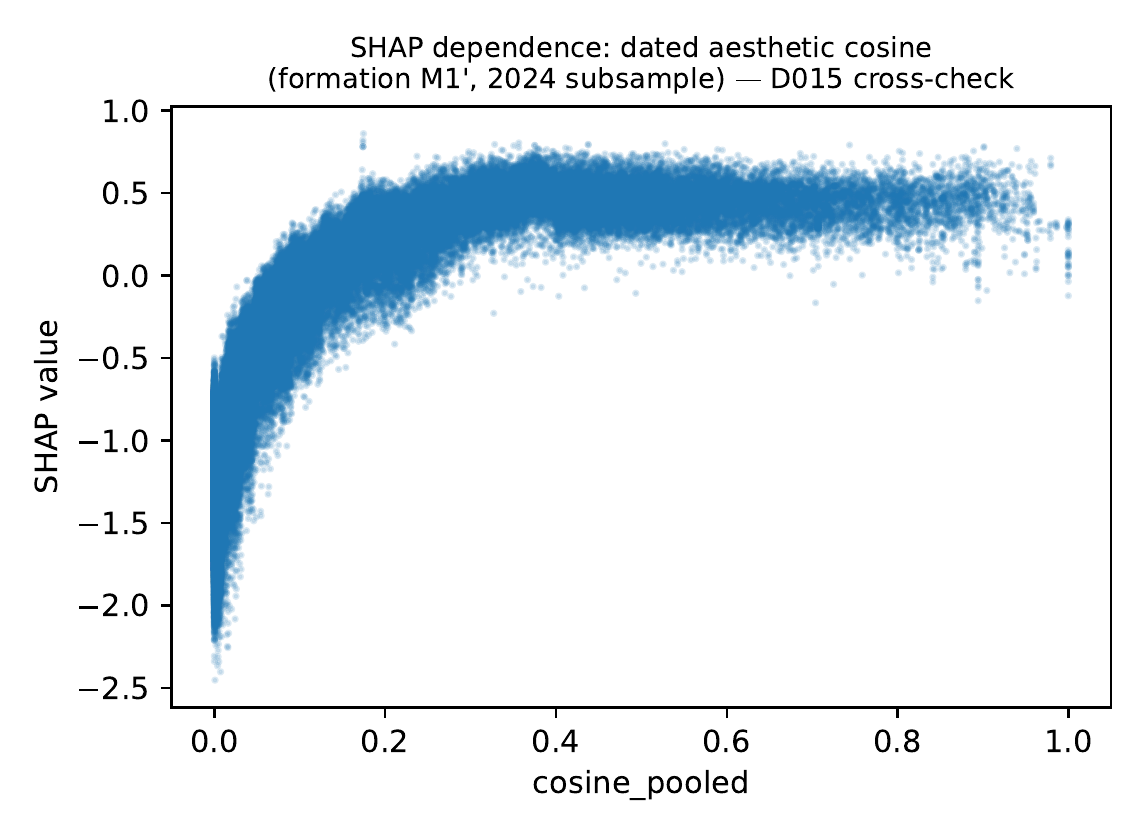
\includegraphics[width=0.9\linewidth,height=\textheight,keepaspectratio]{figures/fig_shap_dependence_cosine.png}
\end{center}

\note{El ejercicio predictivo permite analizar el perfil estético sin
imponer una forma funcional. Para ello, recurrimos a los valores de
Shapley, que descomponen la predicción del XGBoost en las contribuciones
de los distintos predictores. El gráfico representa la contribución de
la similitud estética, en escala de log-odds, para los pares evaluados
en 2024.

El patrón sube con fuerza desde similitudes bajas y después se modera.
Es consistente con el estancamiento del crecimiento del ejercicio
exploratorio y constituye una comprobación descriptiva de lo aprendido
por este modelo. Su utilidad aquí es mostrar que la
\textbf{compatibilidad estética sigue asociada a la formación en un
modelo donde no se fija de antemano una forma funcional.}}

\gdef\roadmapcontent{{\scriptsize \mbox{\color{black!40}Parte 1 · Currículum}\quad \mbox{\color{black!40}Parte 2 · Propuesta docente}\quad \mbox{\color{mDarkTeal}\bfseries Parte 3 · Propuesta investigadora: Creative collaborations}\par}
\vspace{0.8em}
{\large \mbox{\color{black!40}Motivación y pregunta económica}~· \mbox{\color{black!40}Datos y diseño}~· \mbox{\color{mDarkTeal}\bfseries Resultados}~· \mbox{\color{black!40}Conclusiones}\par}
\vspace{0.2em}
\hspace{1.5em}{\normalsize \mbox{\color{black!40}Forma de la asociación}~· \mbox{\color{black!40}Predicción}~· \mbox{\color{mDarkTeal}\bfseries Sensibilidad}\par}}
\end{frame}

\section{Resultados · Sensibilidad}\label{resultados-sensibilidad}

\note{Se ha evaluado la sensibilidad de las estimaciones a la definición
de la respuesta, a diferentes ventanas de actividad, medición de
etiquetas e inferencia. El patrón central sobre afinidad se mantiene. Me
detengo brevemente en la corrección de sesgo debido a la rareza del
evento.}

\begin{frame}{Firth: estabilidad de las estimaciones}
\phantomsection\label{firth-estabilidad-de-las-estimaciones}
\begin{center}

\includegraphics[width=0.89\linewidth,height=\textheight,keepaspectratio]{presentacion_ejercicio_files/mediabag/figures/fig_coef_delta_firth_sebase.pdf}
\end{center}

\textbf{Mayor desplazamiento: 0,23 errores estándar del modelo base.}
Comparación descriptiva de estimaciones puntuales. Todos los
coeficinetes mantienen el signo.

\note{Para ello utilizo el \textbf{modelo logit de Firth} que incorpora
una verosimilitud penalizada para reducir sesgo y mitigar problemas de
separación (que en este caso no se dan). El objeto es comprobar cuánto
cambia el patrón estimado en una muestra con un evento tan infrecuente.

La figura divide la diferencia entre estimaciones por el error estándar
robusto del logit base. Se observa como los desplazamientos son
marginales (el mayor desplazamiento corresponde al índice de Jaccard que
equivale aproximadamente a 0,23 errores estándar en un predictor de
escasa significación sustantiva); además todos los términos conservan su
signo.

Este ejercicio muestra estabilidad de estimaciones puntuales: \textbf{no
hay evidencia de un sesgo relevante asociado a la rareza del evento}.}

\gdef\roadmapcontent{{\scriptsize \mbox{\color{black!40}Parte 1 · Currículum}\quad \mbox{\color{black!40}Parte 2 · Propuesta docente}\quad \mbox{\color{mDarkTeal}\bfseries Parte 3 · Propuesta investigadora: Creative collaborations}\par}
\vspace{0.8em}
{\large \mbox{\color{black!40}Motivación y pregunta económica}~· \mbox{\color{black!40}Datos y diseño}~· \mbox{\color{black!40}Resultados}~· \mbox{\color{mDarkTeal}\bfseries Conclusiones}\par}}
\end{frame}

\section{Conclusiones}\label{conclusiones}

\begin{frame}{Síntesis: afinidad, red y oportunidad}
\phantomsection\label{suxedntesis-afinidad-red-y-oportunidad}
~


\includegraphics[width=0.94\linewidth,height=\textheight,keepaspectratio]{presentacion_ejercicio_files/mediabag/figures/fig_formation_map.pdf}

\note{Antes de concluir, reúno el análisis de los resultados en este
mapa. En horizontal aparece la afinidad estética y en vertical la
cercanía en la red previa. Los paneles comparan una oportunidad conjunta
reciente y una exposición prolongada sin colaboración.

La figura muestra el índice que multiplica la tasa de formación sobre un
\textbf{par de referencia: sin conexión previa, sin afinidad y con una
exposición reciente}.

La interpretación conjunta sugiere que afinidad, distancia relacional y
oportunidad temporal caracterizan configuraciones de formación
distintas.

\begin{itemize}
\item
  Dada una oportunidad reciente, la cercanía en la red multiplica la
  tasa de formación x5; la proximidad estética multiplica x12;
  combinando ambas el factor multiplicativo es x65.
\item
  Un aumento de la exposición al riesgo reduce la tasa de formación.
\end{itemize}

El mapa sintetiza esas asociaciones pero deja abiertas las
explicaciones: puede haber compatibilidad, conexiones o efectos
exposición. Con esta distinción entre evidencia e interpretación paso a
las conclusiones.}
\end{frame}

\begin{frame}{Qué aporta estudiar la formación de colaboraciones}
\phantomsection\label{quuxe9-aporta-estudiar-la-formaciuxf3n-de-colaboraciones}
~

\begin{itemize}
\tightlist
\item
  \textbf{La formación como etapa económica propia}: determina qué
  combinaciones creativas llegan a materializarse.
\item
  \textbf{La hipótesis de distancia óptima exige precisar la etapa y
  contrastar la forma}: los resultados sobre éxito no se trasladan
  automáticamente a la selección de socios.
\item
  \textbf{La siguiente pregunta relaciona selección y rendimiento}:
  quién colabora y qué consigue esa colaboración.
\end{itemize}

\note{Más allá de su aportación metodológica, basada en el conjunto de
riesgo completo y en el uso de técnicas de procesamiento del lenguaje
natural para medir la afinidad entre artistas, el trabajo concibe la
formación de colaboraciones como una etapa diferenciada de la producción
cultural e identifica los factores asociados a su realización.

En los pares analizados, la evidencia es compatible con un requisito de
compatibilidad estética dentro de un conjunto de oportunidades
culturales y relacionales. El contraste flexible evita atribuir una
distancia óptima a lo que podría depender de la especificación del
modelo.

Un resultado generalizable: el análisis del efecto de la afinidad en una
etapa concreta del proceso de producción cultural. \textbf{Estudiar
conjuntamente emparejamiento y rendimiento posterior permitiría
relacionar compatibilidad para la formación con la complementariedad
necesaria para obtener buenos resultados.}}
\end{frame}

\begin{frame}{Alcance y límites de la evidencia}
\phantomsection\label{alcance-y-luxedmites-de-la-evidencia}
~

\begin{longtable}[]{@{}
  >{\raggedright\arraybackslash}p{(\linewidth - 2\tabcolsep) * \real{0.3000}}
  >{\raggedright\arraybackslash}p{(\linewidth - 2\tabcolsep) * \real{0.7000}}@{}}
\toprule\noalign{}
\begin{minipage}[b]{\linewidth}\raggedright
Límite
\end{minipage} & \begin{minipage}[b]{\linewidth}\raggedright
Consecuencia para la interpretación
\end{minipage} \\
\midrule\noalign{}
\endhead
\bottomrule\noalign{}
\endlastfoot
\textbf{Asociaciones} & No se identifican efectos causales \\ \lightrowrule
\textbf{Similitud extrema} & Ocho eventos por encima de 0,90: una
penalización sigue siendo una cuestión abierta \\ \lightrowrule
\textbf{Población y cobertura} & Artistas activos en listas con
metadatos; medidas culturales e institucionales incompletas \\ \lightrowrule
\textbf{Adecuación de la red simulada} & Reproducir el volumen de
vínculos no garantiza reproducir su concentración; la causa de la
discrepancia permanece abierta \\ \lightrowrule
\end{longtable}

\note{La interpretación está sujeta a cuatro límites.

Primero, las estimaciones identifican asociaciones, no efectos causales.

Segundo, la escasez de eventos en la cola de similitud extrema impide
descartar una penalización en esa región.

Tercero, la población está delimitada por la actividad en listas y la
cobertura de metadatos; además, las etiquetas y la definición de la
escena incorporan ruido, y los sellos reflejan solo un canal
institucional.

Finalmente, la adecuación de la red es clave para justificar la
independencia condicional del modelo diádico. El modelo base reproduce
el volumen de vínculos, pero no tanto su concentración, lo que requiere
reevaluar con especificación flexibles. Su diagnóstico continua junto
con las extensiones sustantiva}
\end{frame}

\begin{frame}[plain]{}
\phantomsection\label{section}
\begin{tikzpicture}[remember picture,overlay]
  \fill[SlateTealDeck] (current page.south west) rectangle (current page.north east);
  \node at (current page.center) {\usebeamerfont{title}\color{white}Agradecimientos};
\end{tikzpicture}
\end{frame}

\begin{frame}
\titlepage
\end{frame}




\end{document}
